\documentclass[xetex,mathserif,serif,handout]{beamer}

\usepackage{xunicode}
\usepackage{xltxtra}
\usepackage{color}
\usepackage{url}
\usepackage{listings}
\usepackage{fontspec}
\usepackage{geometry}
\usepackage{lastpage}
\usepackage{fancyhdr}
\usepackage{amsmath}
\usepackage{amsthm}
\usepackage{amssymb}
\usepackage{blkarray}
\usepackage{multicol}
\usepackage{relsize}

\definecolor{solarized@base03}{HTML}{002B36}
\definecolor{solarized@base02}{HTML}{073642}
\definecolor{solarized@base01}{HTML}{586e75}
\definecolor{solarized@base00}{HTML}{657b83}
\definecolor{solarized@base0}{HTML}{839496}
\definecolor{solarized@base1}{HTML}{93a1a1}
\definecolor{solarized@base2}{HTML}{EEE8D5}
\definecolor{solarized@base3}{HTML}{FDF6E3}
\definecolor{solarized@yellow}{HTML}{B58900}
\definecolor{solarized@orange}{HTML}{CB4B16}
\definecolor{solarized@red}{HTML}{DC322F}
\definecolor{solarized@magenta}{HTML}{D33682}
\definecolor{solarized@violet}{HTML}{6C71C4}
\definecolor{solarized@blue}{HTML}{268BD2}
\definecolor{solarized@cyan}{HTML}{2AA198}
\definecolor{solarized@green}{HTML}{859900}
\definecolor{yaleblue}{HTML}{0E4C92}

\setbeamertemplate{navigation symbols}{}
% \setbeamerfont{title}{family=\old}
% \setbeamerfont{author}{family=\tfont}%
% \setbeamerfont{frametitle}{family=\oldA}
% \setbeamerfont{date}{family=\dfont}

\setbeamertemplate{itemize items}{--}
\setbeamercolor*{item}{fg=black}

\defaultfontfeatures{Mapping=tex-text}
\hypersetup{pdfstartview={FitH}}

\newcommand{\old}[1]{\fontspec[Alternate=1,Ligatures={Common}]{Hoefler Text}\fontsize{18pt}{30pt}\selectfont #1}%
\newcommand{\oldA}[1]{\fontspec[Alternate=1,Ligatures={Common, Rare}]{Hoefler Text}\fontsize{12pt}{15pt}\selectfont #1}%
\newcommand{\oldB}[1]{\fontspec[Ligatures={Common}]{Didot}\fontsize{12pt}{15pt}\color{solarized@base02}\selectfont #1}%
\newcommand{\tfont}[1]{\fontspec[Alternate=1,Ligatures={Common}]{Hoefler Text}\fontsize{12pt}{20pt}\selectfont #1}%
\newcommand{\dfont}[1]{\fontspec[Ligatures={Common}]{Didot}\fontsize{12pt}{12pt}\selectfont #1}%

\newcommand{\minimize}{\mathop{\mathrm{minimize}}}
\newcommand{\argmin}{\mathop{\mathrm{arg\,min}}}
\newcommand{\argmax}{\mathop{\mathrm{arg\,max}}}
\newcommand{\st}{\mathop{\mathrm{subject\,\,to}}}

\newcommand\independent{\protect\mathpalette{\protect\independenT}{\perp}}
\def\independenT#1#2{\mathrel{\rlap{$#1#2$}\mkern2mu{#1#2}}}

\setlength{\parindent}{0pt}
\setlength{\parskip}{12pt}

\setromanfont [Ligatures={Common}, Numbers={OldStyle}, Variant=01,
 BoldFont={LinLibertine_RB.otf},
 ItalicFont={LinLibertine_RI.otf},
 BoldItalicFont={LinLibertine_RBI.otf}
 ]{LinLibertine_R.otf}



\begin{document}

%%%%%%%%%%%%%%%%%%%%%%%%%%%%%%%%%%%%%%%%%%%%%%%%%%%
\begin{frame}[fragile] \frametitle{}

\vfill

{\fontsize{0.7cm}{0cm}\selectfont Lecture 22 \\\vspace{0.2cm}
The Generalized Lasso}\\\vspace{0.5cm}
07 December 2015

\vspace{2cm}

\begin{minipage}{0.6\textwidth}
Taylor B. Arnold \\
Yale Statistics  \\
STAT 312/612
\end{minipage}
\hfill
\begin{minipage}{0.3\textwidth}\raggedleft

\includegraphics[scale=0.3]{../yale-logo.png}
\end{minipage}%

\end{frame}

%%%%%%%%%%%%%%%%%%%%%%%%%%%%%%%%%%%%%%%%%%%%%%%%%%%
\begin{frame}[fragile] \frametitle{}

{\color{yaleblue}\fontsize{16pt}{20pt}\selectfont Class Notes}

\begin{itemize}
\item Midterm II - Due today
\item Problem Set 7 - Available now, please hand in by the 16th
\end{itemize}

\end{frame}

%%%%%%%%%%%%%%%%%%%%%%%%%%%%%%%%%%%%%%%%%%%%%%%%%%%
\begin{frame}
  \frametitle{Motivation}
  \footnotesize

  \begin{itemize}
  \item Today I am going to introduce the generalized lasso. Rather than just giving a
      theoretical description without any data-driven motivation, I have instead
      modified a talk I gave on pricing personal home insurance. \pause
  \item At a high level, my primary focus was understanding what factors contribute
      to the relative risk of insuring a person, vehicle, house, boat, apartment, ect. \pause
  \item Examples of covariates
    used to study risk include: a person's credit score, an automobile's price,
    and the method of heating used within a house. \pause
  \item One particularly important aspect of risk in personal insurance is the location
    where the insured entity (home or automobile) is located. \pause
  \item For instance, homes located in flood or fire zones have obvious, direct
      effects on their risk due to location.\pause
  \item Location also plays an indirect role on risk, as it is highly correlated with
    other variables such as income, age, occupation, and vehicle usage, many of which
    are hard to reliably collect and verify.
  \end{itemize}

\end{frame}

%%%%%%%%%%%%%%%%%%%%%%%%%%%%%%%%%%%%%%%%%%%%%%%%%%%
\begin{frame}
  \frametitle{Insurance territory models}
  \footnotesize

  Given the special and important nature of location, we created
  \magenta{territory models} to
  describe the relative insurance risk due to location. Specifically, this
  is a process of mapping locations in a given area into a prediction of
  its riskiness (i.e., price). \pause

  \medskip

  Specific issues that arise in constructing territory models include:
  \begin{itemize}
  \item Dealing with data that are available at different degrees
    of granularity (state, city, zip, census block...),
    with the smaller levels providing more segmentation at the expense of
    noisier predictions. Furthermore, some data is only available at certain resolutions. \pause
  \item Implementation concerns, regulatory restrictions, and the need for
    interpretability makes it difficult to use complex estimators like
    kriging. \pause
  \item Determining whether to treat each region as a fixed effect (with its
    own intercept), or if prediction should be done primarily on the metadata attached
    to a given region.
  \end{itemize}

\end{frame}

%%%%%%%%%%%%%%%%%%%%%%%%%%%%%%%%%%%%%%%%%%%%%%%%%%%
\begin{frame}
  \frametitle{Insurance territory models, cont.}
  \footnotesize

  \begin{itemize}
  \item We use aggregated industry data, for each specific coverage specific
    (house fires, auto collision, \ldots), to build our territory models.
  \item Unfortunately, due to licensing restrictions and the very competitive
    nature of personal insurance I am not able to present results from our
    industry or internal data.
  \item However, I do have access to a small set of data which almost perfectly resembles
    the industry data we use, for the
    \cyan{home theft} coverage within the city of Chicago.
  \end{itemize}

\end{frame}


%%%%%%%%%%%%%%%%%%%%%%%%%%%%%%%%%%%%%%%%%%%%%%%%%%%
\begin{frame}
  \frametitle{Chicago Crime Data}
  \footnotesize

  \begin{itemize}
  \item There exists an open data feed, which gives
    several basic pieces of information about individual reported
    crimes.\footnote{https://data.cityofchicago.org/Public-Safety/Crimes-2001-to-present\\}
  \item This includes a specific latitude and longitude of the incident, the
    date and time of the report, and primary categorization of the crime.
  \item \magenta{Idea:} Spatially join the burglary crimes
    to census block groups, and divide this number by the number of households in
    the block group. By modeling this, it should yield the relative territorial risk of
    insuring a home against burglary.
  \end{itemize}

\end{frame}


%%%%%%%%%%%%%%%%%%%%%%%%%%%%%%%%%%%%%%%%%%%%%%%%%%%
\begin{frame}
  \frametitle{Chicago Crime Data, Observed.}
  \footnotesize

  \begin{columns}[T]
    \begin{column}{.5\textwidth}
     \begin{block}{}
  On the right, are the observed values of the response number of burglaries
  between 2012 divided by the number of households. Red is the highest
  percentage and white is the lowest percentage. \\

  \medskip

  We clearly see spatial trends, but also notice that at this level of granularity,
  there is still quite a bit of noise.

  \medskip

  Still, if we were interested purely in a machine learning type algorithm to predict
  the proportion of burglaries in the year 2013, simply using the observed in 2012
  will be a very good guess.

    \end{block}
    \end{column}
    \begin{column}{.5\textwidth}
    \vspace{-0.3cm}
  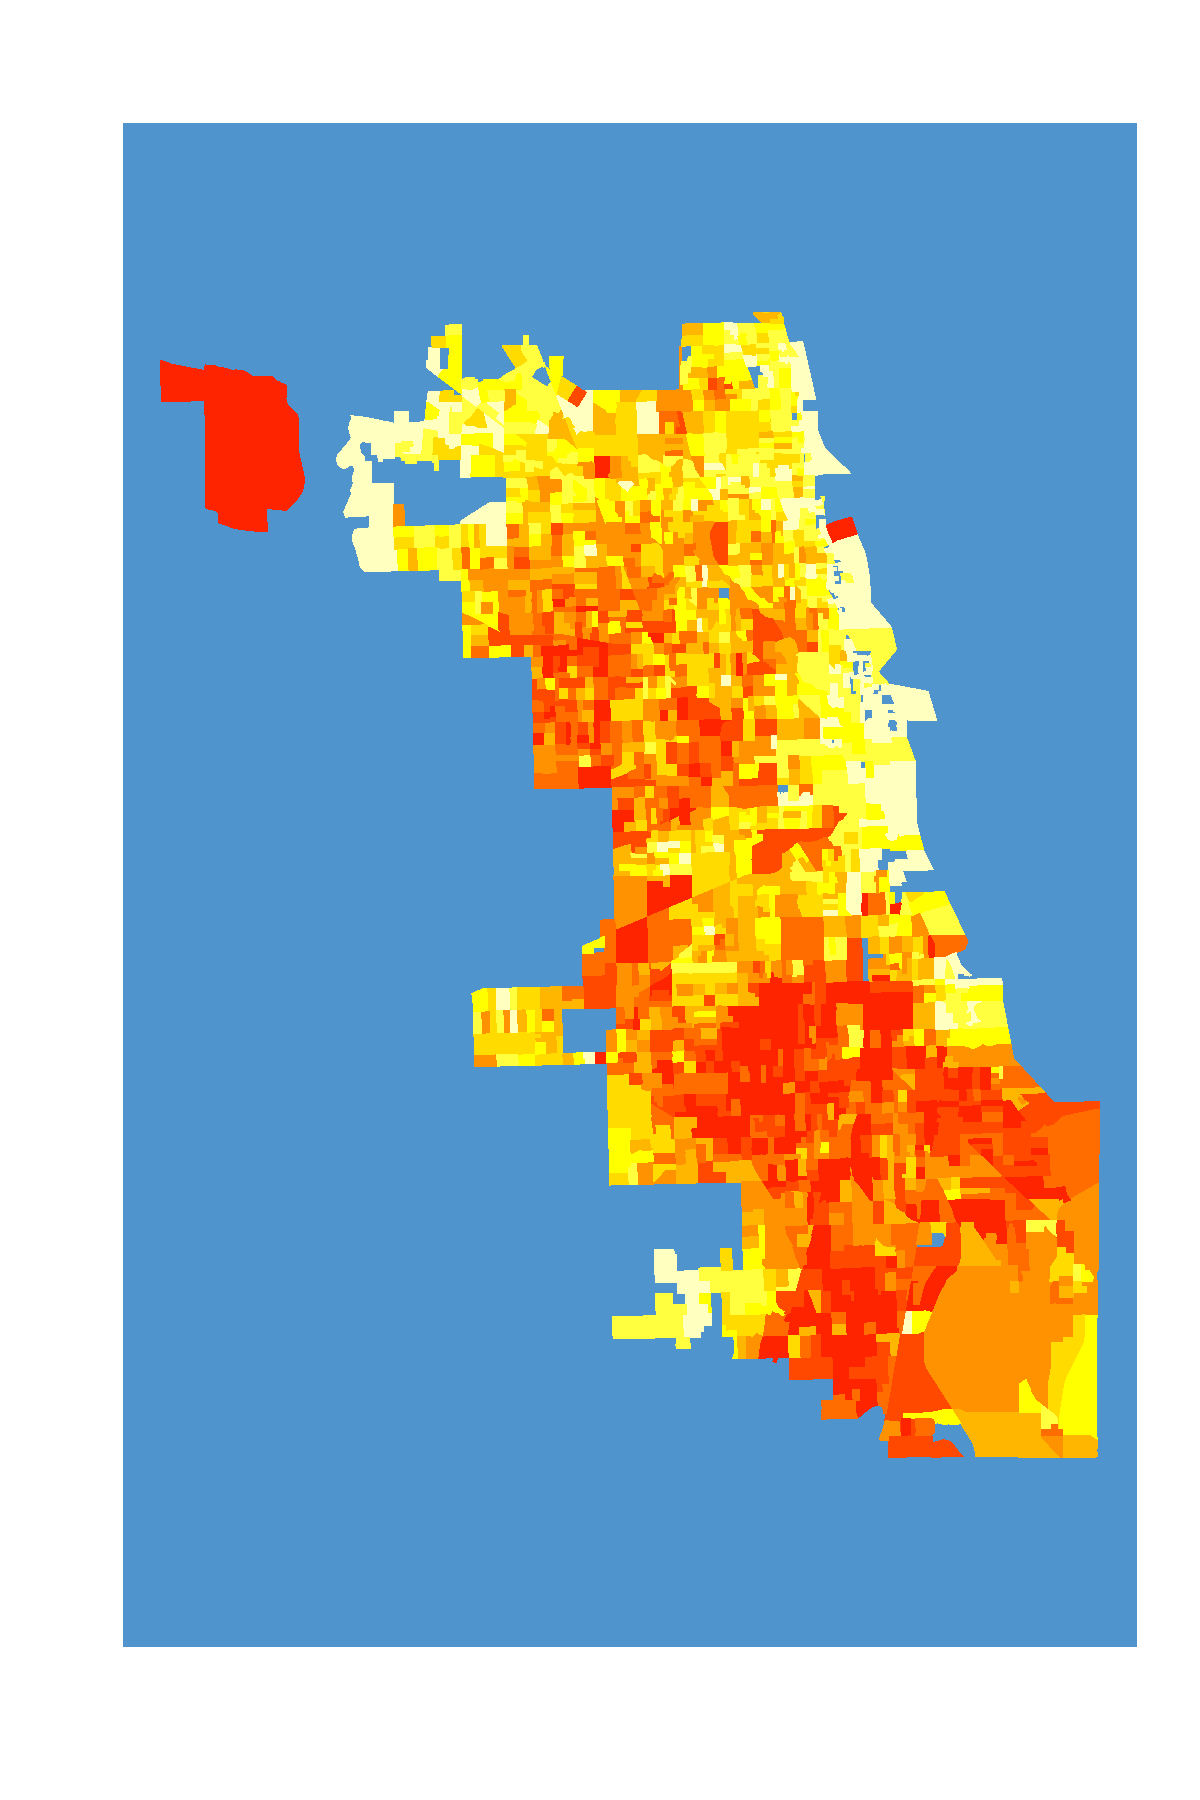
\includegraphics[height=3.6in]{img/chi1}
    \end{column}
  \end{columns}

\end{frame}


%%%%%%%%%%%%%%%%%%%%%%%%%%%%%%%%%%%%%%%%%%%%%%%%%%%
\begin{frame}
  \frametitle{Spatial Clustering: Concepts and goals}
  \footnotesize

  Rather than using the observed values, we need to cluster the regions
  together to form larger clumps of similar risk. This is necessary for the following
  reasons:
  \begin{itemize}
  \item If we use territory as a fixed effect (possibly even as an interaction),
  need to reduce the number of regions\pause
  \item For business purposes and regulatory issues, need to have a model which
  is easier to understand and manage\pause
  \item To avoid over-fitting to the mix of demographics in a region, since will not
  necessarily insure a homogeneous mix within a block group\pause
  \end{itemize}
  In particular, we need a spatial clustering algorithm which is locally adaptive. That
  is, we want the algorithm to locally determine the number of clusters needed to fit
  the data `well'.

  \medskip

  Since we need adaptability, it makes sense to try to formalize a statistical
  model which will impose the form of sparsity we are trying to construct.


\end{frame}

%%%%%%%%%%%%%%%%%%%%%%%%%%%%%%%%%%%%%%%%%%%%%%%%%%%
\begin{frame}
  \frametitle{Theoretical model: Basic set-up}
  \small

  Consider the output of independent random variables observed on the nodes of a graph,
    such as:
  \vspace{-0.3in}

  \begin{center}
  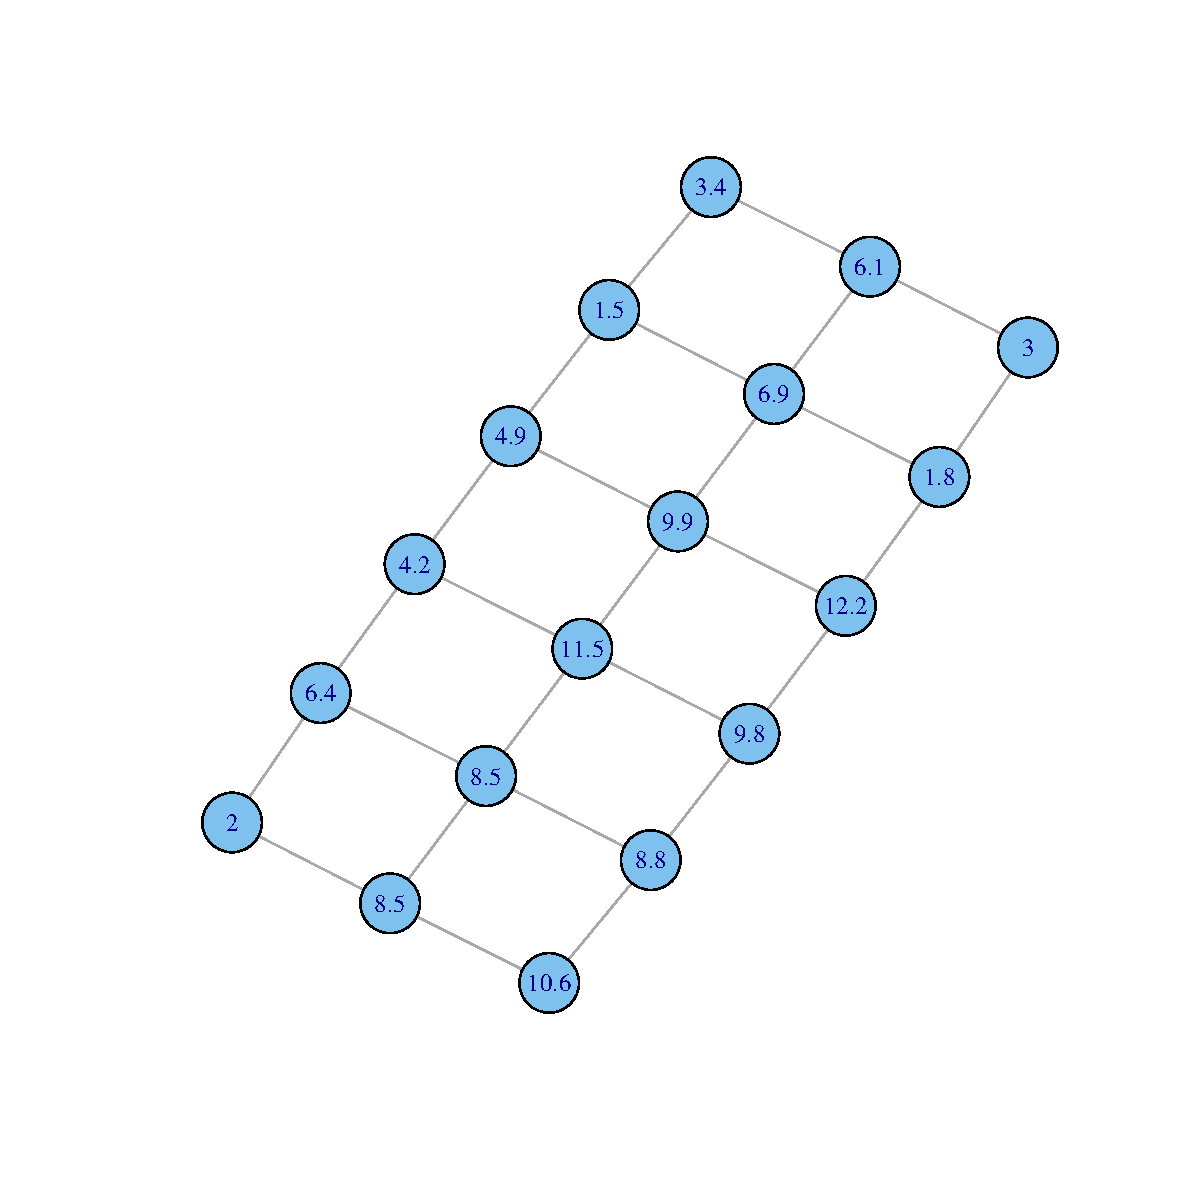
\includegraphics[height=3in]{img/graph_plain}
  \end{center}

\end{frame}


%%%%%%%%%%%%%%%%%%%%%%%%%%%%%%%%%%%%%%%%%%%%%%%%%%%
\begin{frame}
  \frametitle{Theoretical model: Basic set-up, cont.}
  \small

  If we have reason to believe that the true means of the nodes are
  \magenta{piecewise constant}
  along the edges, a reasonable partition of this graph is given by:

  \vspace{-0.3in}

  \begin{center}
  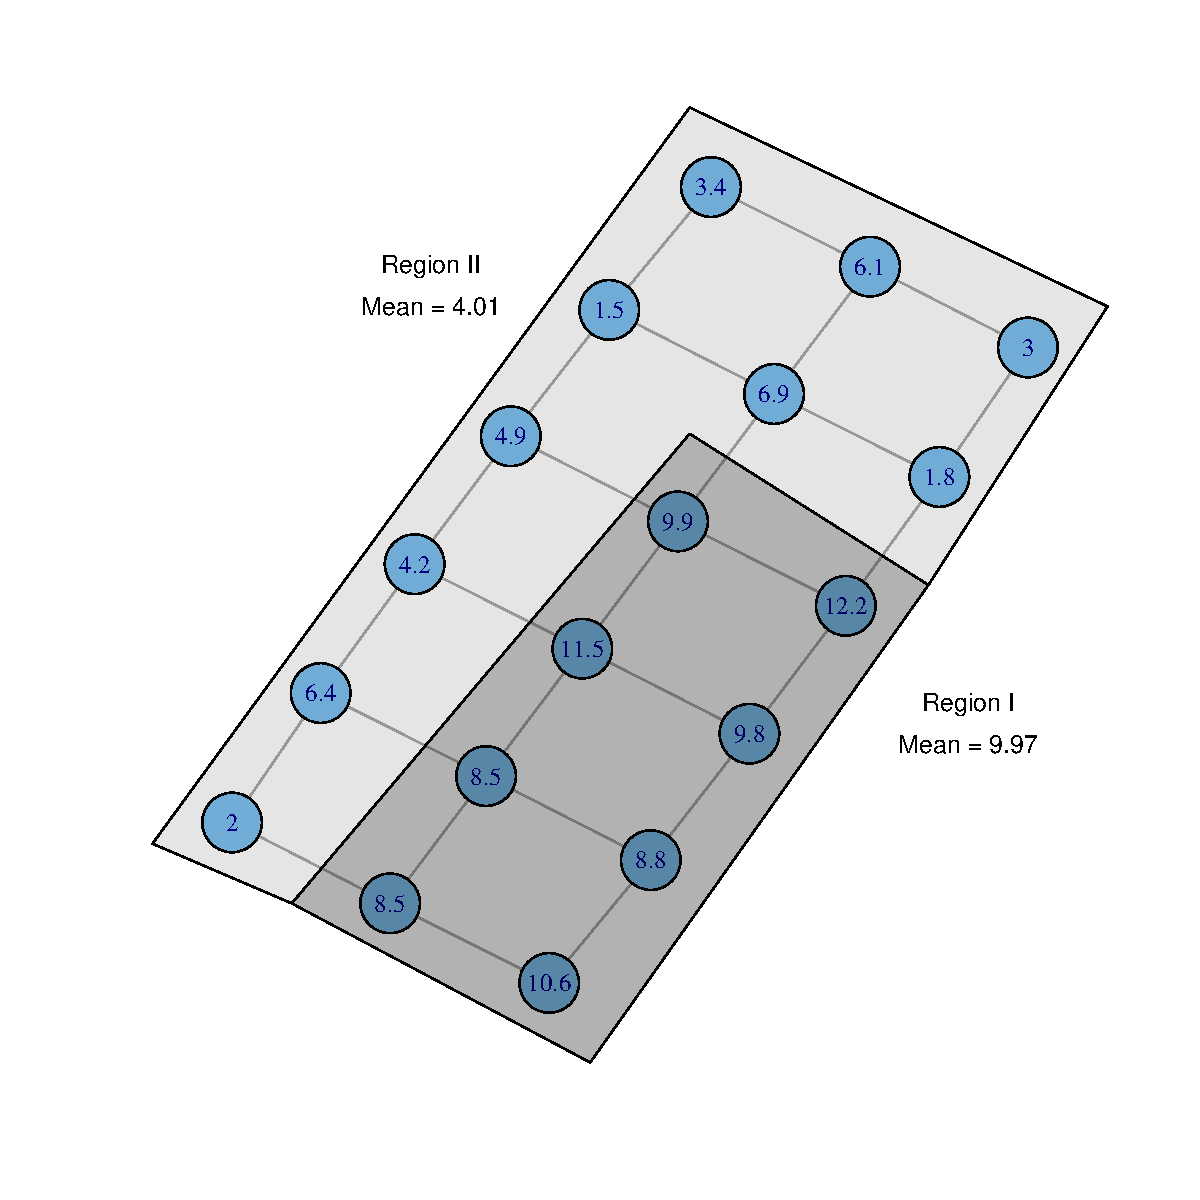
\includegraphics[height=3in]{img/graph_region}
  \end{center}

\end{frame}

%%%%%%%%%%%%%%%%%%%%%%%%%%%%%%%%%%%%%%%%%%%%%%%%%%%
\begin{frame}
  \frametitle{The fused lasso}
  \footnotesize

  The fused lasso is a statistical estimator for estimating this structure on arbitrary graphs,
  defined as the minimizer of the residual sum of squares, plus an $\ell_1$ penalty term for edges
  with discordant mean predictions:
  \begin{align}
    \widehat{\beta}_{fused} &= \argmin_{\beta} \, \frac{1}{2}|| y - \beta ||_2^2 +
          \lambda \cdot \sum_{(i,j) \in \text{edges}} | \beta_i - \beta_j |
  \end{align}
  \pause As with the traditional lasso, the tuning parameter $\lambda$ controls the degree of smoothness
  imposed on the estimator. We can re-write this condition compactly in terms of the of the oriented
  incidence matrix $D$; this matrix has a row for every edge and a column for every node, with
  elements $\pm1$ to indicate the nodes in an edge (each row has one positive and one negative
  entry, for our purposes the choice is arbitrary):
  \begin{align}
    \widehat{\beta}_{fused} &= \argmin_{\beta} \, \frac{1}{2}|| y - \beta ||_2^2 +
           \lambda \cdot || D \beta ||_1
  \end{align}


\end{frame}

%%%%%%%%%%%%%%%%%%%%%%%%%%%%%%%%%%%%%%%%%%%%%%%%%%%
\begin{frame}[fragile] \frametitle{}
  \frametitle{Simple 1D Example}
  \small

  The simplest example of the fused lasso applies the algorithm to ordered data (corresponding
  to a chain graph). From this perspective, the fused lasso is essentially solving the classic
  change point problem, which has a wide range of applications.

Notice that this case can be written as:
\begin{align*}
|| y - \beta ||_2^2 + \lambda \cdot \sum_{i=1}^{n-1} || \beta_{i} - \beta_{i+1} ||_1
\end{align*}

\end{frame}

%%%%%%%%%%%%%%%%%%%%%%%%%%%%%%%%%%%%%%%%%%%%%%%%%%%
\begin{frame}[fragile] \frametitle{}

We can write this as:
\begin{align*}
|| y - \beta ||_2^2 + \lambda \cdot || D \beta ||_1
\end{align*}
For the aforementioned matrix $D$. In the case of $n=5$, this looks like:
\begin{align*}
D &= \left(\begin{array}{ccccc}
1 & -1 & 0 & 0 & 0\\
0 & 1 & -1 & 0 & 0\\
0 & 0 & 1 & -1 & 0\\
0 & 0 & 0 & 1 & -1\\
\end{array}\right)
\end{align*}

\end{frame}

%%%%%%%%%%%%%%%%%%%%%%%%%%%%%%%%%%%%%%%%%%%%%%%%%%%
\begin{frame}
  \frametitle{Simple 1D Example}
  \small

  Applying this to data gives a fit like the following:
  \vspace{-0.3in}

  \begin{center}
  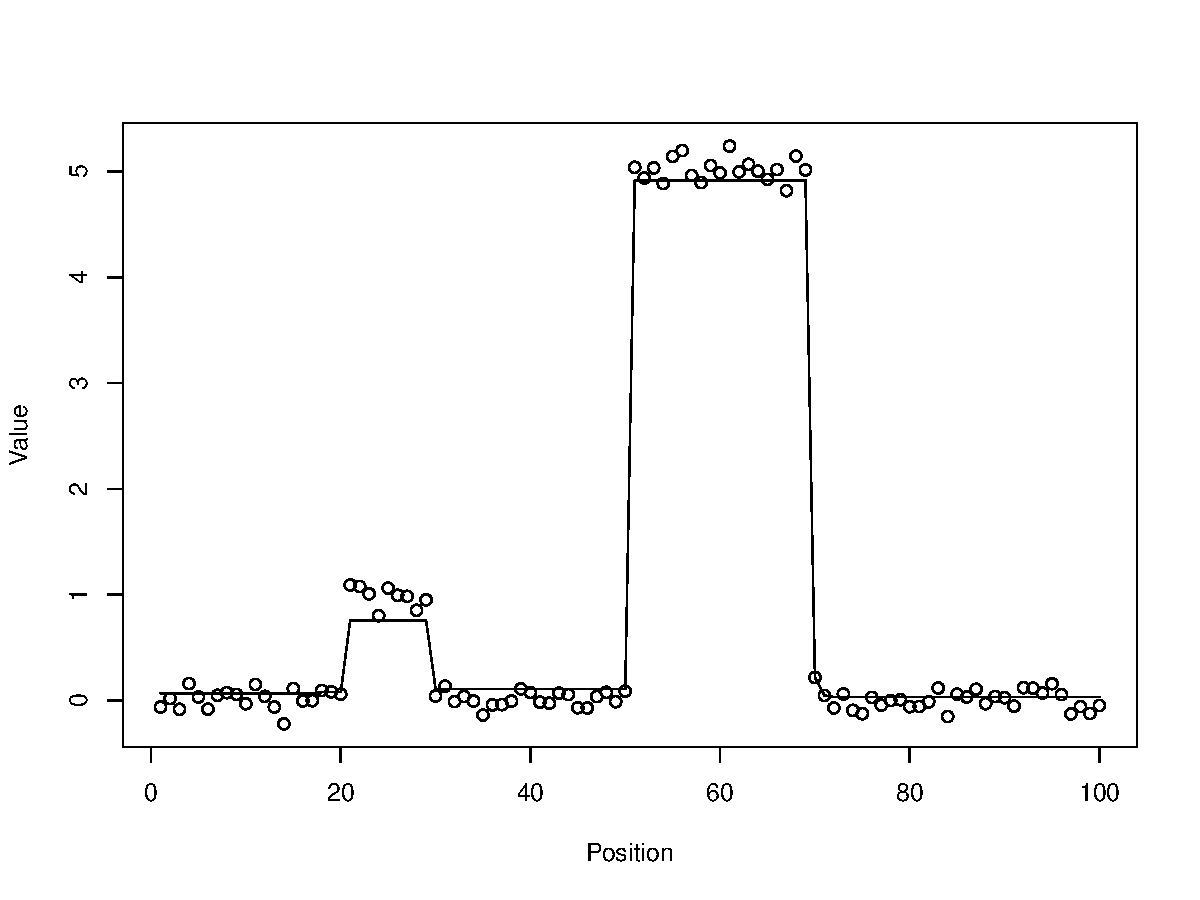
\includegraphics[height=2.5in]{img/simple_fused}
  \end{center}

\end{frame}


%%%%%%%%%%%%%%%%%%%%%%%%%%%%%%%%%%%%%%%%%%%%%%%%%%%
\begin{frame}
  \frametitle{Simple 2D Example}
  \small

  A small 2d is shown below (dark green is a low value, pink is a high value), for several
  values of the $\lambda$ tuning parameter.

  \vspace{-0in}

  \begin{center}
  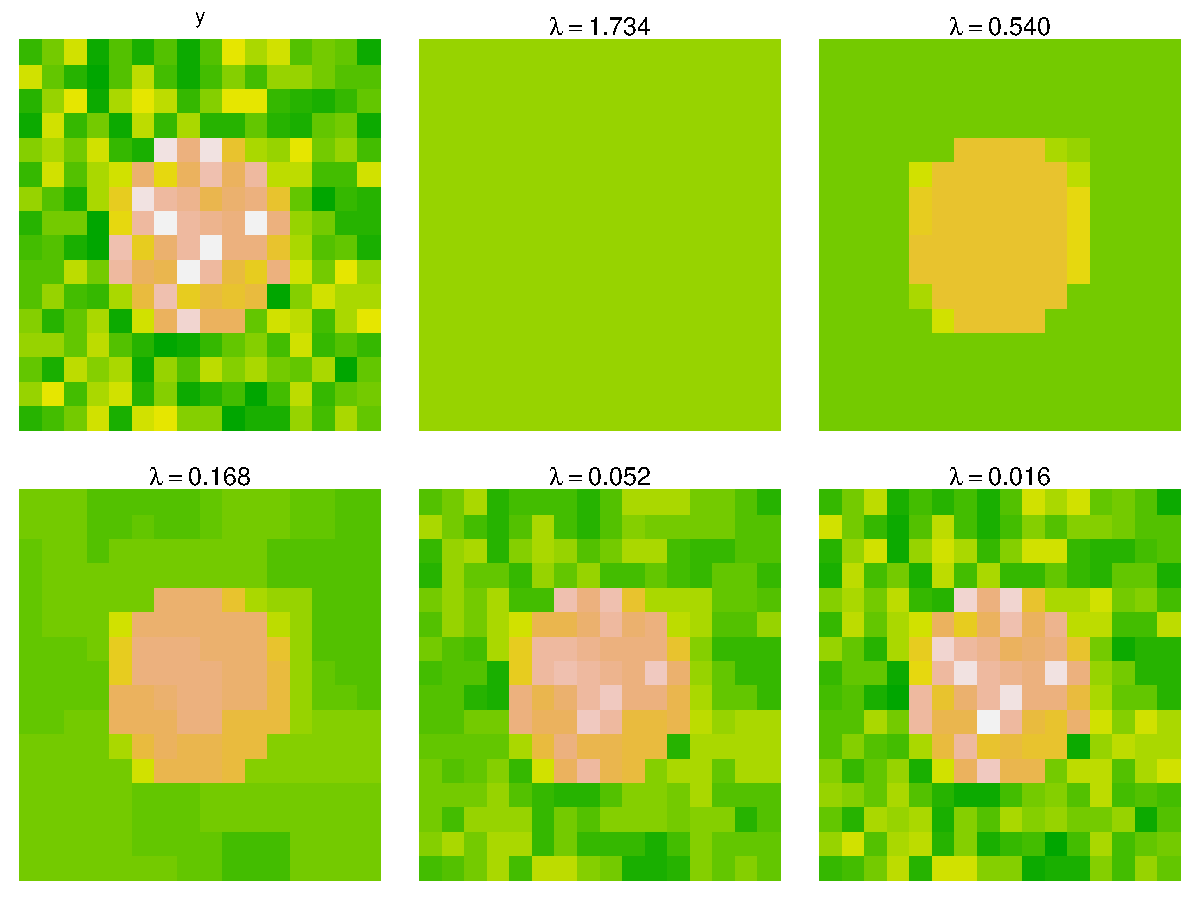
\includegraphics[height=2.5in]{img/simple_2dfused}
  \end{center}

\end{frame}


%%%%%%%%%%%%%%%%%%%%%%%%%%%%%%%%%%%%%%%%%%%%%%%%%%%
\begin{frame}
  \frametitle{The Dual problem}
  \footnotesize

  The fused lasso optimisation problem is convex; therefore we can solve it by translating
  to the dual problem. Re-writing the fused lasso as:
  \begin{align}
  \argmin_{\beta} \, \frac{1}{2}|| y - \beta ||_2^2 +
           \lambda \cdot || z ||_1, \, \, \text{s.t.} \, \, z = D\beta
  \end{align}
  \pause The Lagrangian becomes:
  \begin{align}
  \Lambda(\beta, z, u) &= \frac{1}{2} || y - \beta ||_2^2 + \lambda ||z||_1 + u^{t} (D\beta - z) \\
  &= \frac{1}{2} || y - \beta ||_2^2 +u^{t} D\beta + \lambda ||z||_1 - u^{t} z
  \end{align}

\end{frame}

%%%%%%%%%%%%%%%%%%%%%%%%%%%%%%%%%%%%%%%%%%%%%%%%%%%
\begin{frame}
  \frametitle{Graphical depiction of the Lagrangian}
  \small

  For a visual understanding of the dual problem we can visualize the
  Lagrangian solution as a saddle point\footnote{www.convexoptimization.com \\}

  \vspace{-0in}

  \begin{center}
  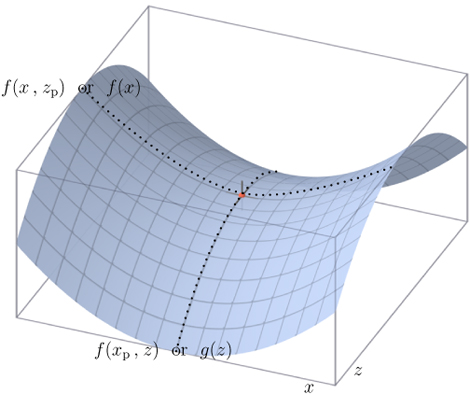
\includegraphics[height=2.5in]{img/saddle}
  \end{center}

\end{frame}

%%%%%%%%%%%%%%%%%%%%%%%%%%%%%%%%%%%%%%%%%%%%%%%%%%%
\begin{frame}
  \frametitle{The Dual problem, cont.}
  \footnotesize

  The dual function $g(u)$, is the infimum of $\Lambda$ over $\beta$ and $z$.
  \begin{align}
  \Lambda(\beta, z, u) &= \frac{1}{2} || y - \beta ||_2^2 +u^{t} D\beta + \lambda ||z||_1 - u^{t} z
  \end{align}
  Notice that if $||u||_\infty > \lambda$ then $g(u) = -\infty$. Otherwise, the infimum over
  $z$ of $\lambda ||z||_1 - u^t z$ is equal to zero.

\end{frame}

%%%%%%%%%%%%%%%%%%%%%%%%%%%%%%%%%%%%%%%%%%%%%%%%%%%
\begin{frame}
  \frametitle{The Dual problem, cont.}
  \footnotesize

  In the case when $||u||_\infty \leq \lambda$, the value of $g(u)$ depends only on the
  $\beta$ infimum, given by:
  \begin{align}
  \min_{\beta} \, \frac{1}{2} || y - \beta ||_2^2 +u^{t} D\beta = - \frac{1}{2} || y - D^T u ||_2^2
  \end{align}
  Finally, the dual problem is to find the maximum of $g(u)$ over all $u$. We can wrap all
  of the conditions up nicely by stating the dual problem as:
  \begin{align}
  \min_u \frac{1}{2} || y - D^T u ||_2^2, \, \text{s.t.} \, \, \, ||u||_\infty \leq \lambda
  \end{align}
  Given a solution to this, there is a corresponding solution to primal problem by the
  relationship $\widehat{\beta}_\lambda = y - D^T \widehat{u}_\lambda$.

\end{frame}

%%%%%%%%%%%%%%%%%%%%%%%%%%%%%%%%%%%%%%%%%%%%%%%%%%%
\begin{frame}
  \frametitle{Concept behind the dual fused lasso problem}
  \footnotesize

  \begin{itemize}
  \item Using duality, we have converted an $\ell_1$ constrained problem on the nodes of
  the graph to an $\ell_\infty$ constrained problem on the edges of the graph.
  \item For most graphs (connected, non-trees), this transformation has increased the
  dimensionality of the problem. For large values of $\lambda$, the solution space
  may have a very high dimensionality.
  \item \magenta{Good news:} There exists a solution to the dual
  problem where the coordinates of $u$ are piecewise linear with respect to $\lambda$.
  \end{itemize}

\end{frame}

%%%%%%%%%%%%%%%%%%%%%%%%%%%%%%%%%%%%%%%%%%%%%%%%%%%
\begin{frame}
  \frametitle{Analytic path solution}
  \footnotesize

  For $\lambda_0 = \infty$, the dual problem reduces to a least squares
  optimization. If $D^t$ is not full column rank, there is not a unique
  least squares solution. However, we can define a canonical solution by
  using the Moore-Penrose pseudo-inverse:
  \begin{align}
  \widehat{u}_{\lambda_0} = (DD^T)^{+} D y \label{leastsqr}
  \end{align}
  In the path solution, the first `break point' occurs at:
  \begin{align}
  \lambda_1 = || \widehat{u}_{\lambda_0} ||_\infty
  \end{align}
  At this point, the coordinate of $u$ on the boundary is set to $\pm \lambda$,
  and the other coordinates are determined by solving (\ref{leastsqr}), with
  the corresponding row of $D$ removed.

\end{frame}

%%%%%%%%%%%%%%%%%%%%%%%%%%%%%%%%%%%%%%%%%%%%%%%%%%%
\begin{frame}
  \frametitle{Computational notes}
  \footnotesize

  \begin{itemize}
  \item In the classical lasso, the path starts from simplest model and works towards
  more complex ones. The dual solution is the opposite; we need to compute the full
  least squares solution before even starting the path.\pause
  \item At the start of the path solution, the algorithm is only moving around in the
  null space of $D^T$. It is not until enough edges (corresponding the coordinates of
  u) sit on the $\lambda$ boundary to disconnect the graph, that we see non-trival
  solutions in the primal problem.\pause
  \item The least squares problem is being constantly solved, with one variable removed
  in each step. We can save the QR-decomposition of $D^T$, and utilize Given's rotations
  to drastically increase the speed of this process.\pause
  \item For most graphs of interest, the matrix $D$ will be sparse (and perhaps banded,
  for 1D problems). Taking advantage of sparse matrix libraries can increase the
  computational speed further.\pause
  \item Once the graph in the primal problem becomes disconnected, the dual problem
  likewise become decoupled. Keeping track of the graph problems allows for efficiencies
  by solving the problem independently on each disconnected component.
  \end{itemize}

\end{frame}

%%%%%%%%%%%%%%%%%%%%%%%%%%%%%%%%%%%%%%%%%%%%%%%%%%%
\begin{frame}
  \frametitle{Implementation}
  \footnotesize

  The R package \magenta{genlasso}\footnote{Ryan Tibshirani and
  Taylor Arnold (2014). genlasso: Path algorithm for generalized lasso problems.
  R package version 1.2.\\}, available on CRAN, provides an implementation of this
  path algorithm. Some particularly notable features of the package:
  \begin{itemize}
  \item Works for a generic $D$ matrix, not just the fused lasso.
  \item Incorporates the computational points in the previous slide.
  \item Functionality for iterating an incomplete path, filebacking large problems,
  cross-validation techniques to tune the $\lambda$, and the ability to include a
  design matrix $X$.
  \item A standard set of S3 methods for plotting, summarizing, predicting, and
  extracting coefficients from a genlasso object.
  \end{itemize}

\end{frame}

%%%%%%%%%%%%%%%%%%%%%%%%%%%%%%%%%%%%%%%%%%%%%%%%%%%
\begin{frame}

  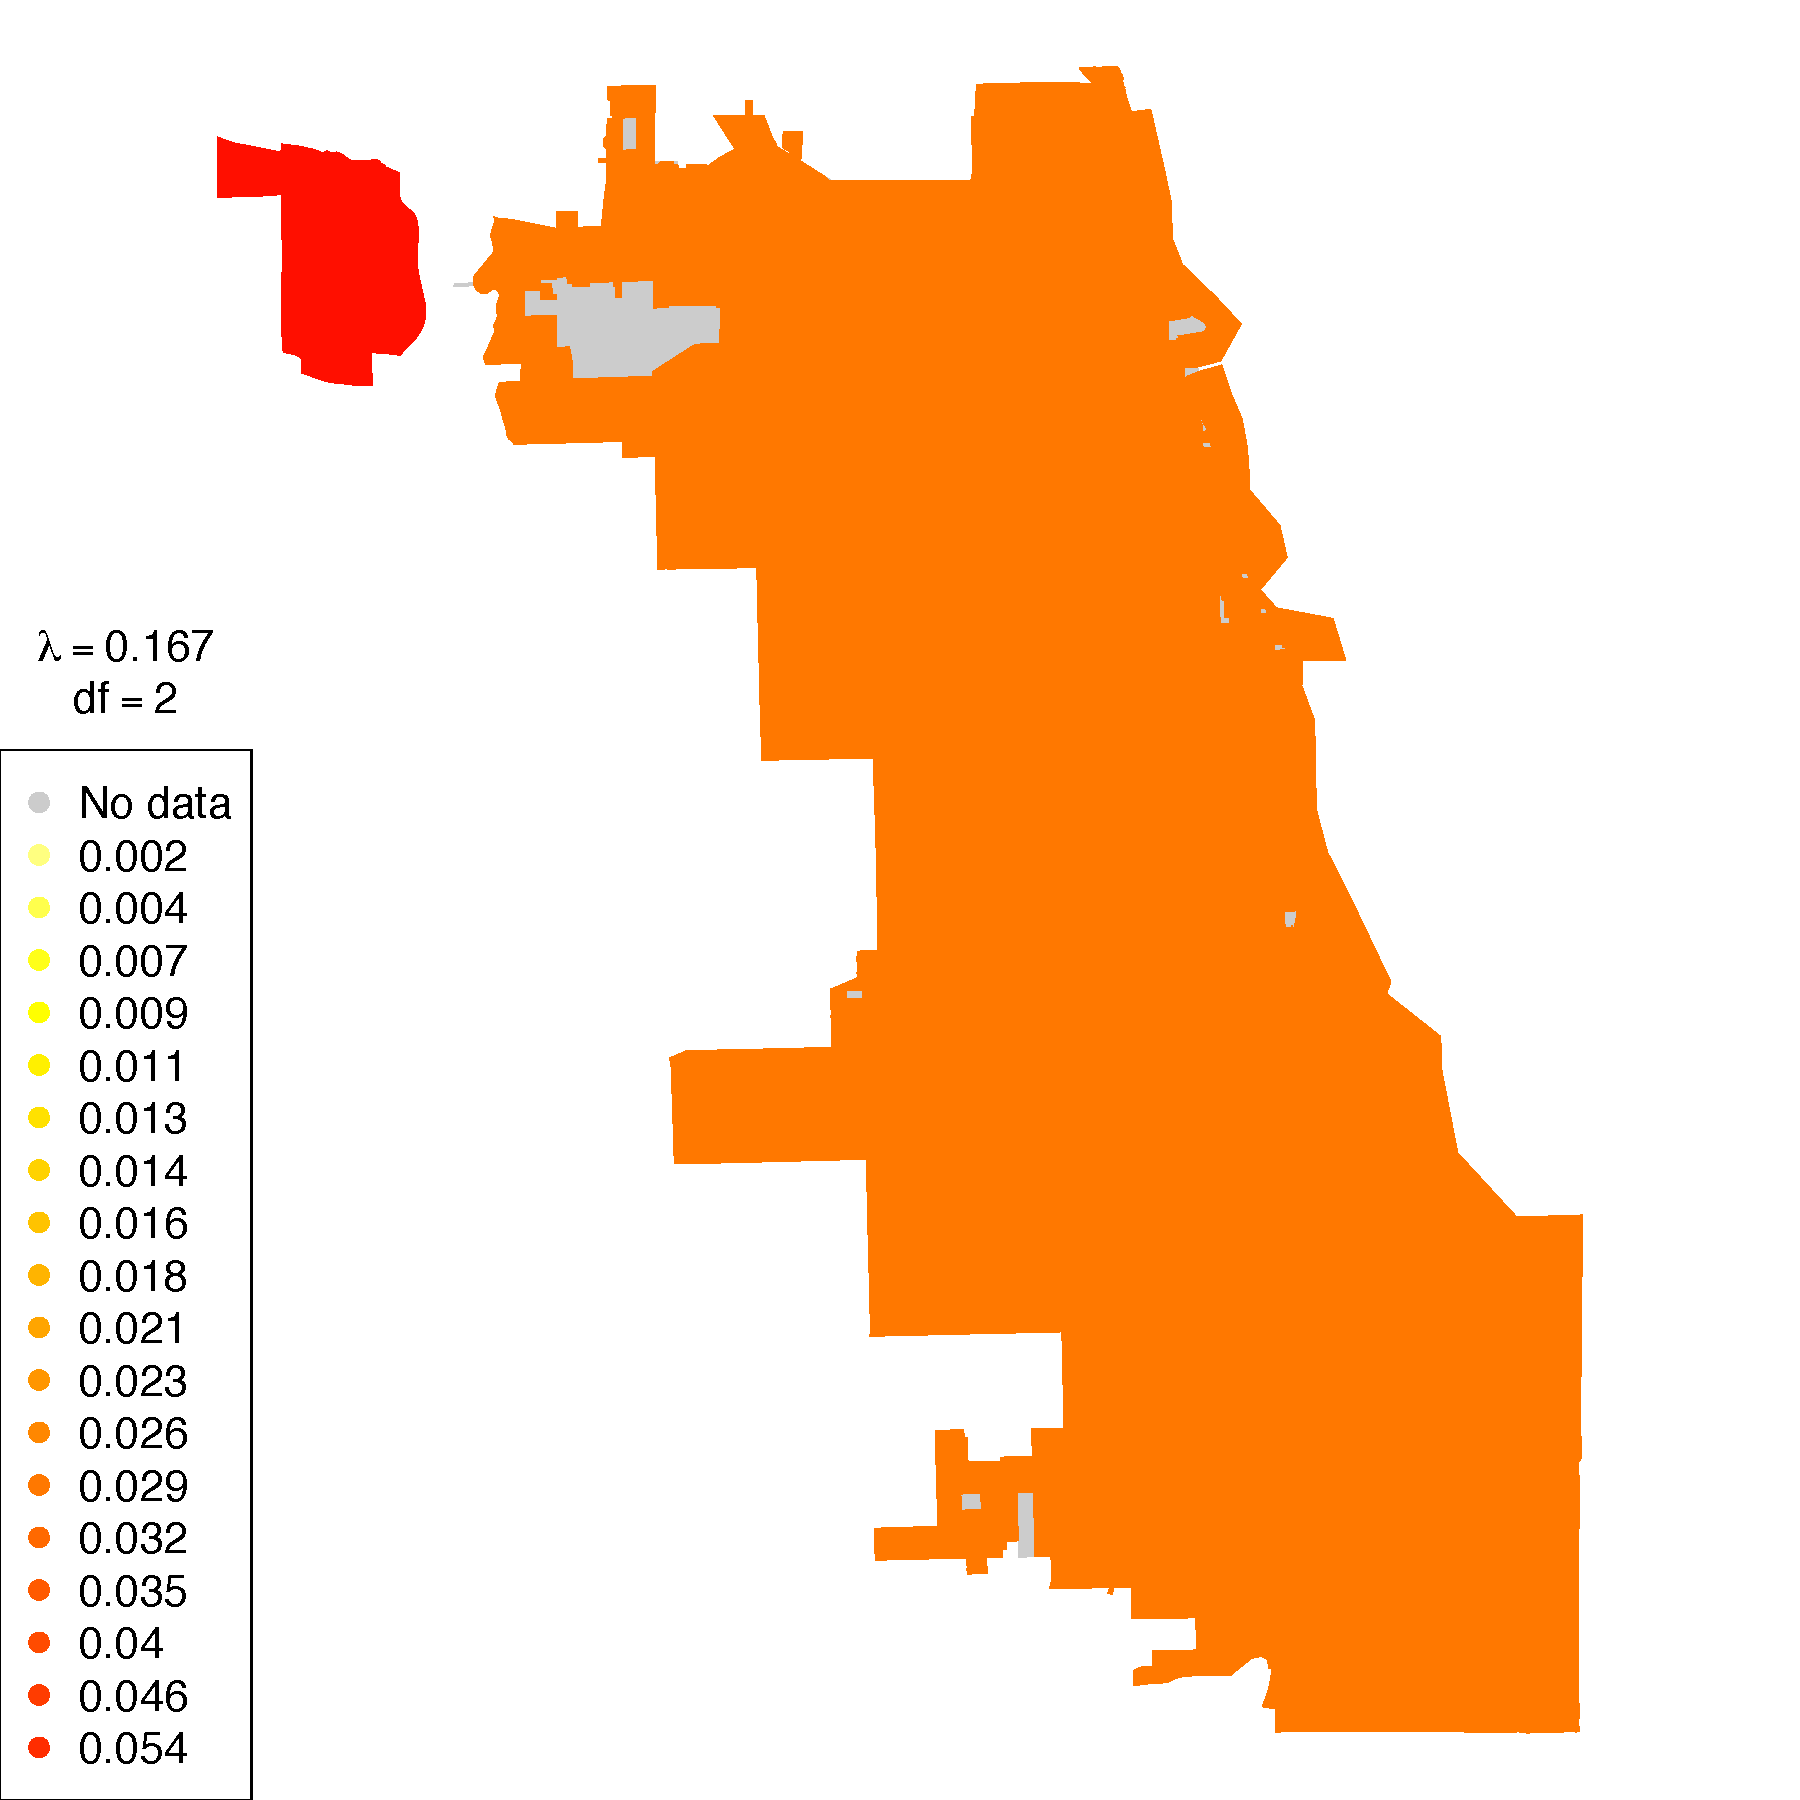
\includegraphics[height=\textheight]{img/chicago_rob_2df.pdf}

\end{frame}

%%%%%%%%%%%%%%%%%%%%%%%%%%%%%%%%%%%%%%%%%%%%%%%%%%%
\begin{frame}

  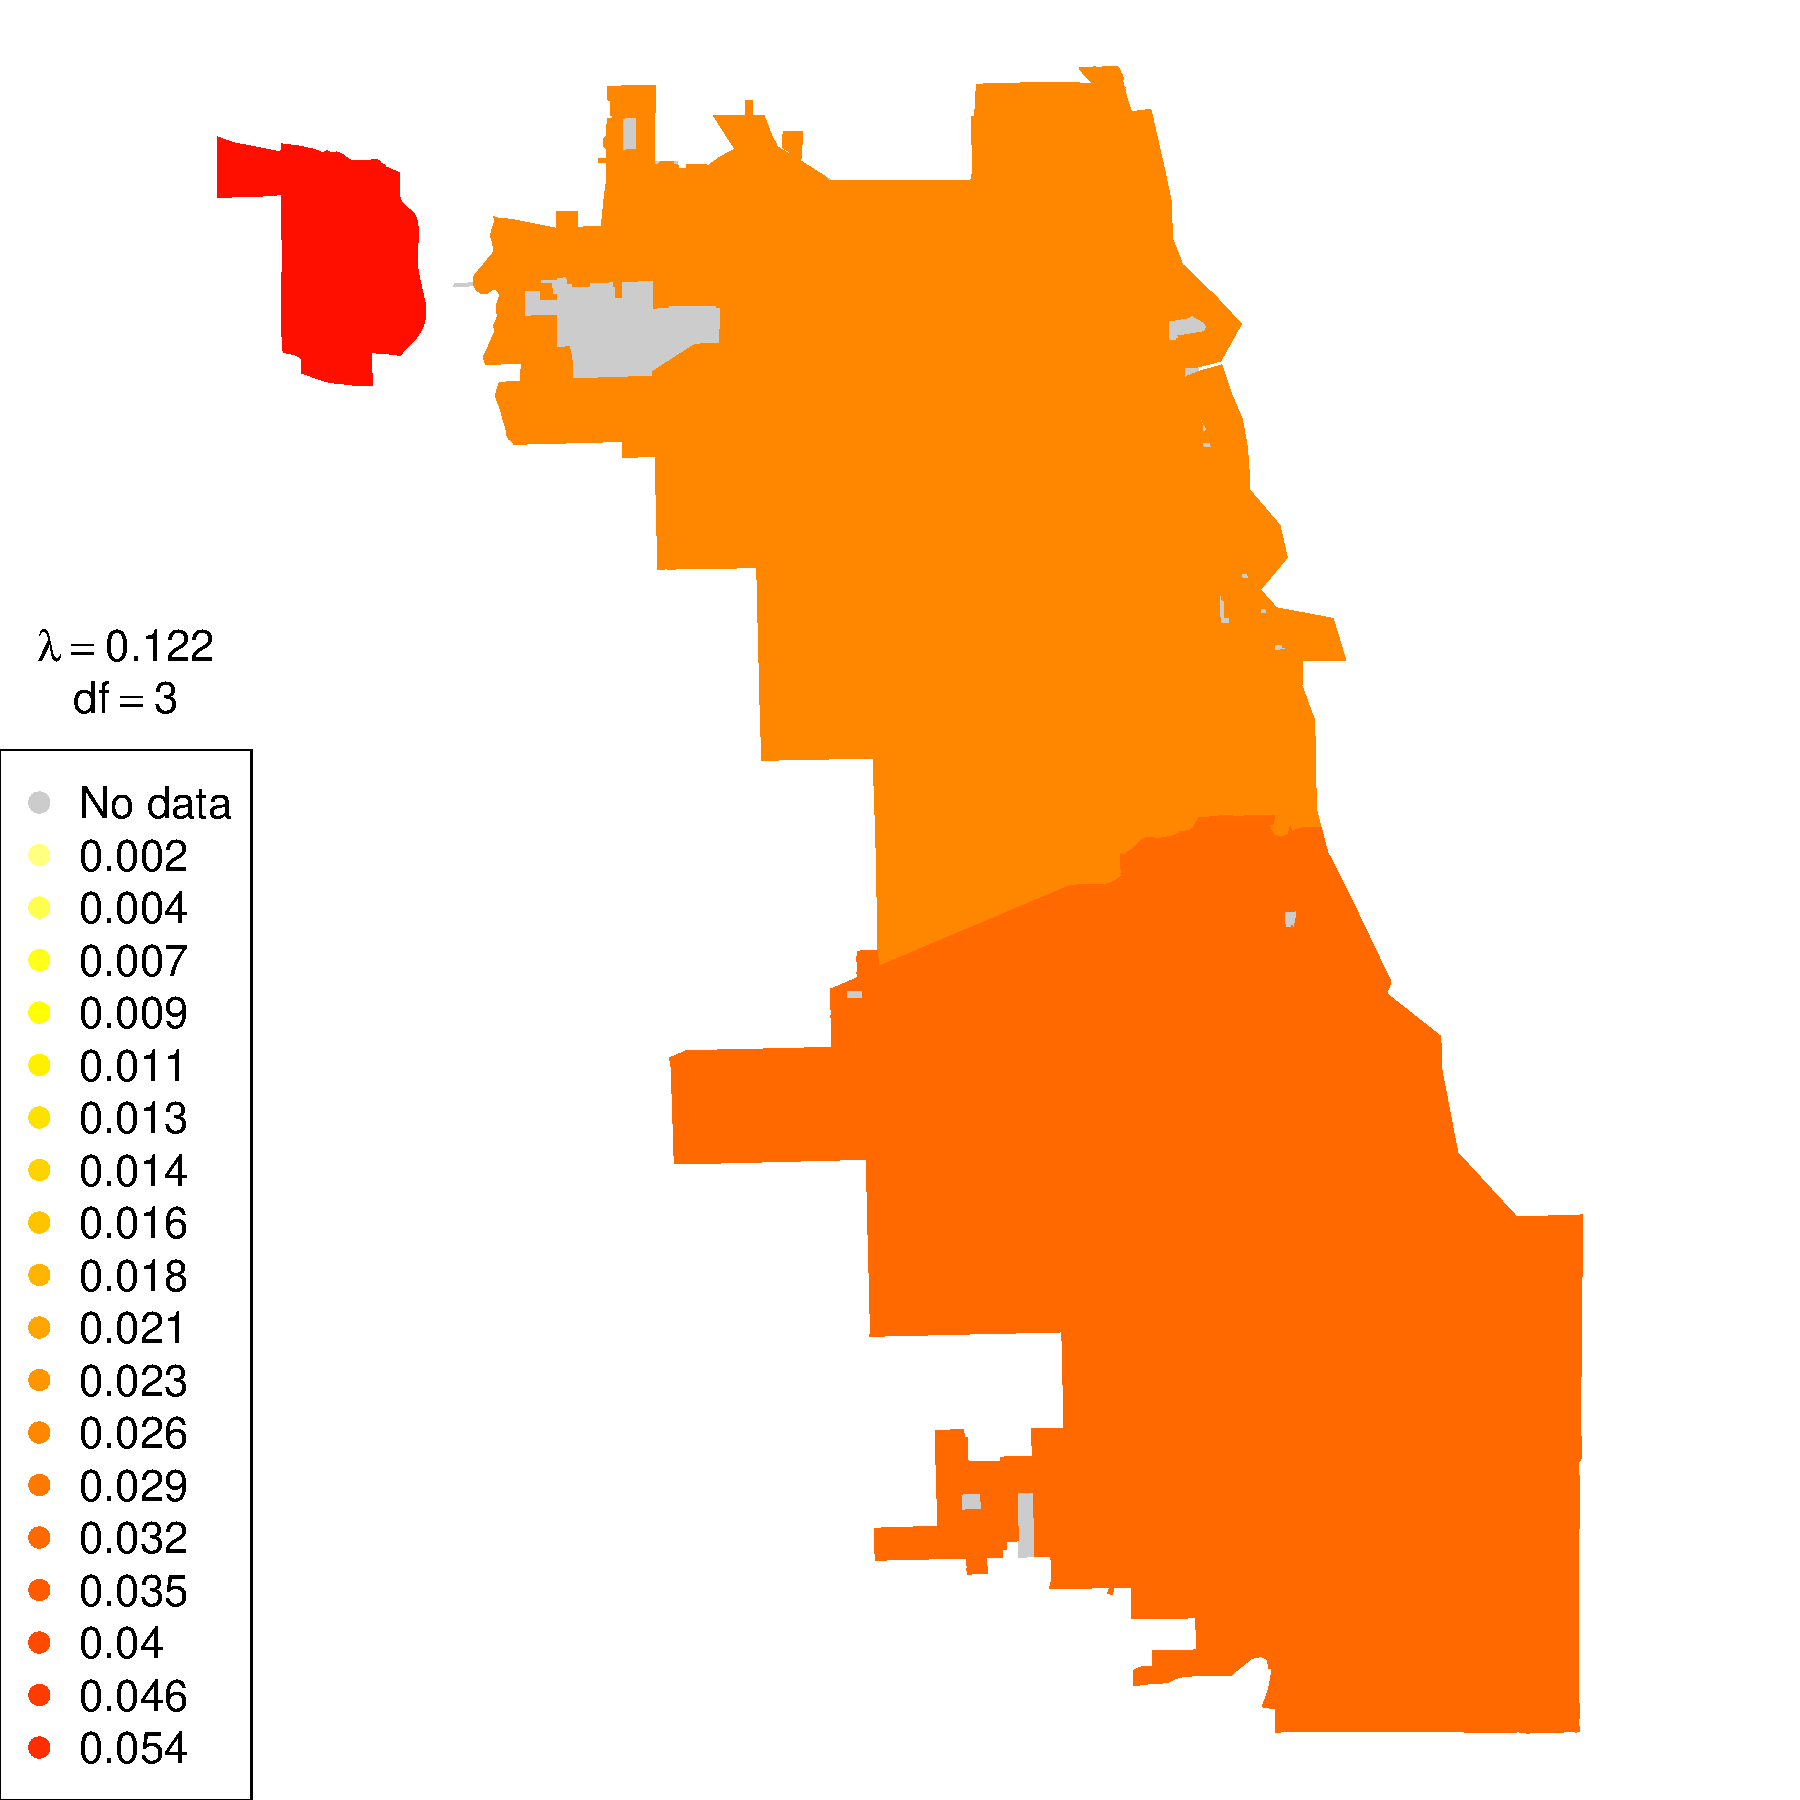
\includegraphics[height=\textheight]{img/chicago_rob_3df.pdf}

\end{frame}

%%%%%%%%%%%%%%%%%%%%%%%%%%%%%%%%%%%%%%%%%%%%%%%%%%%
\begin{frame}

  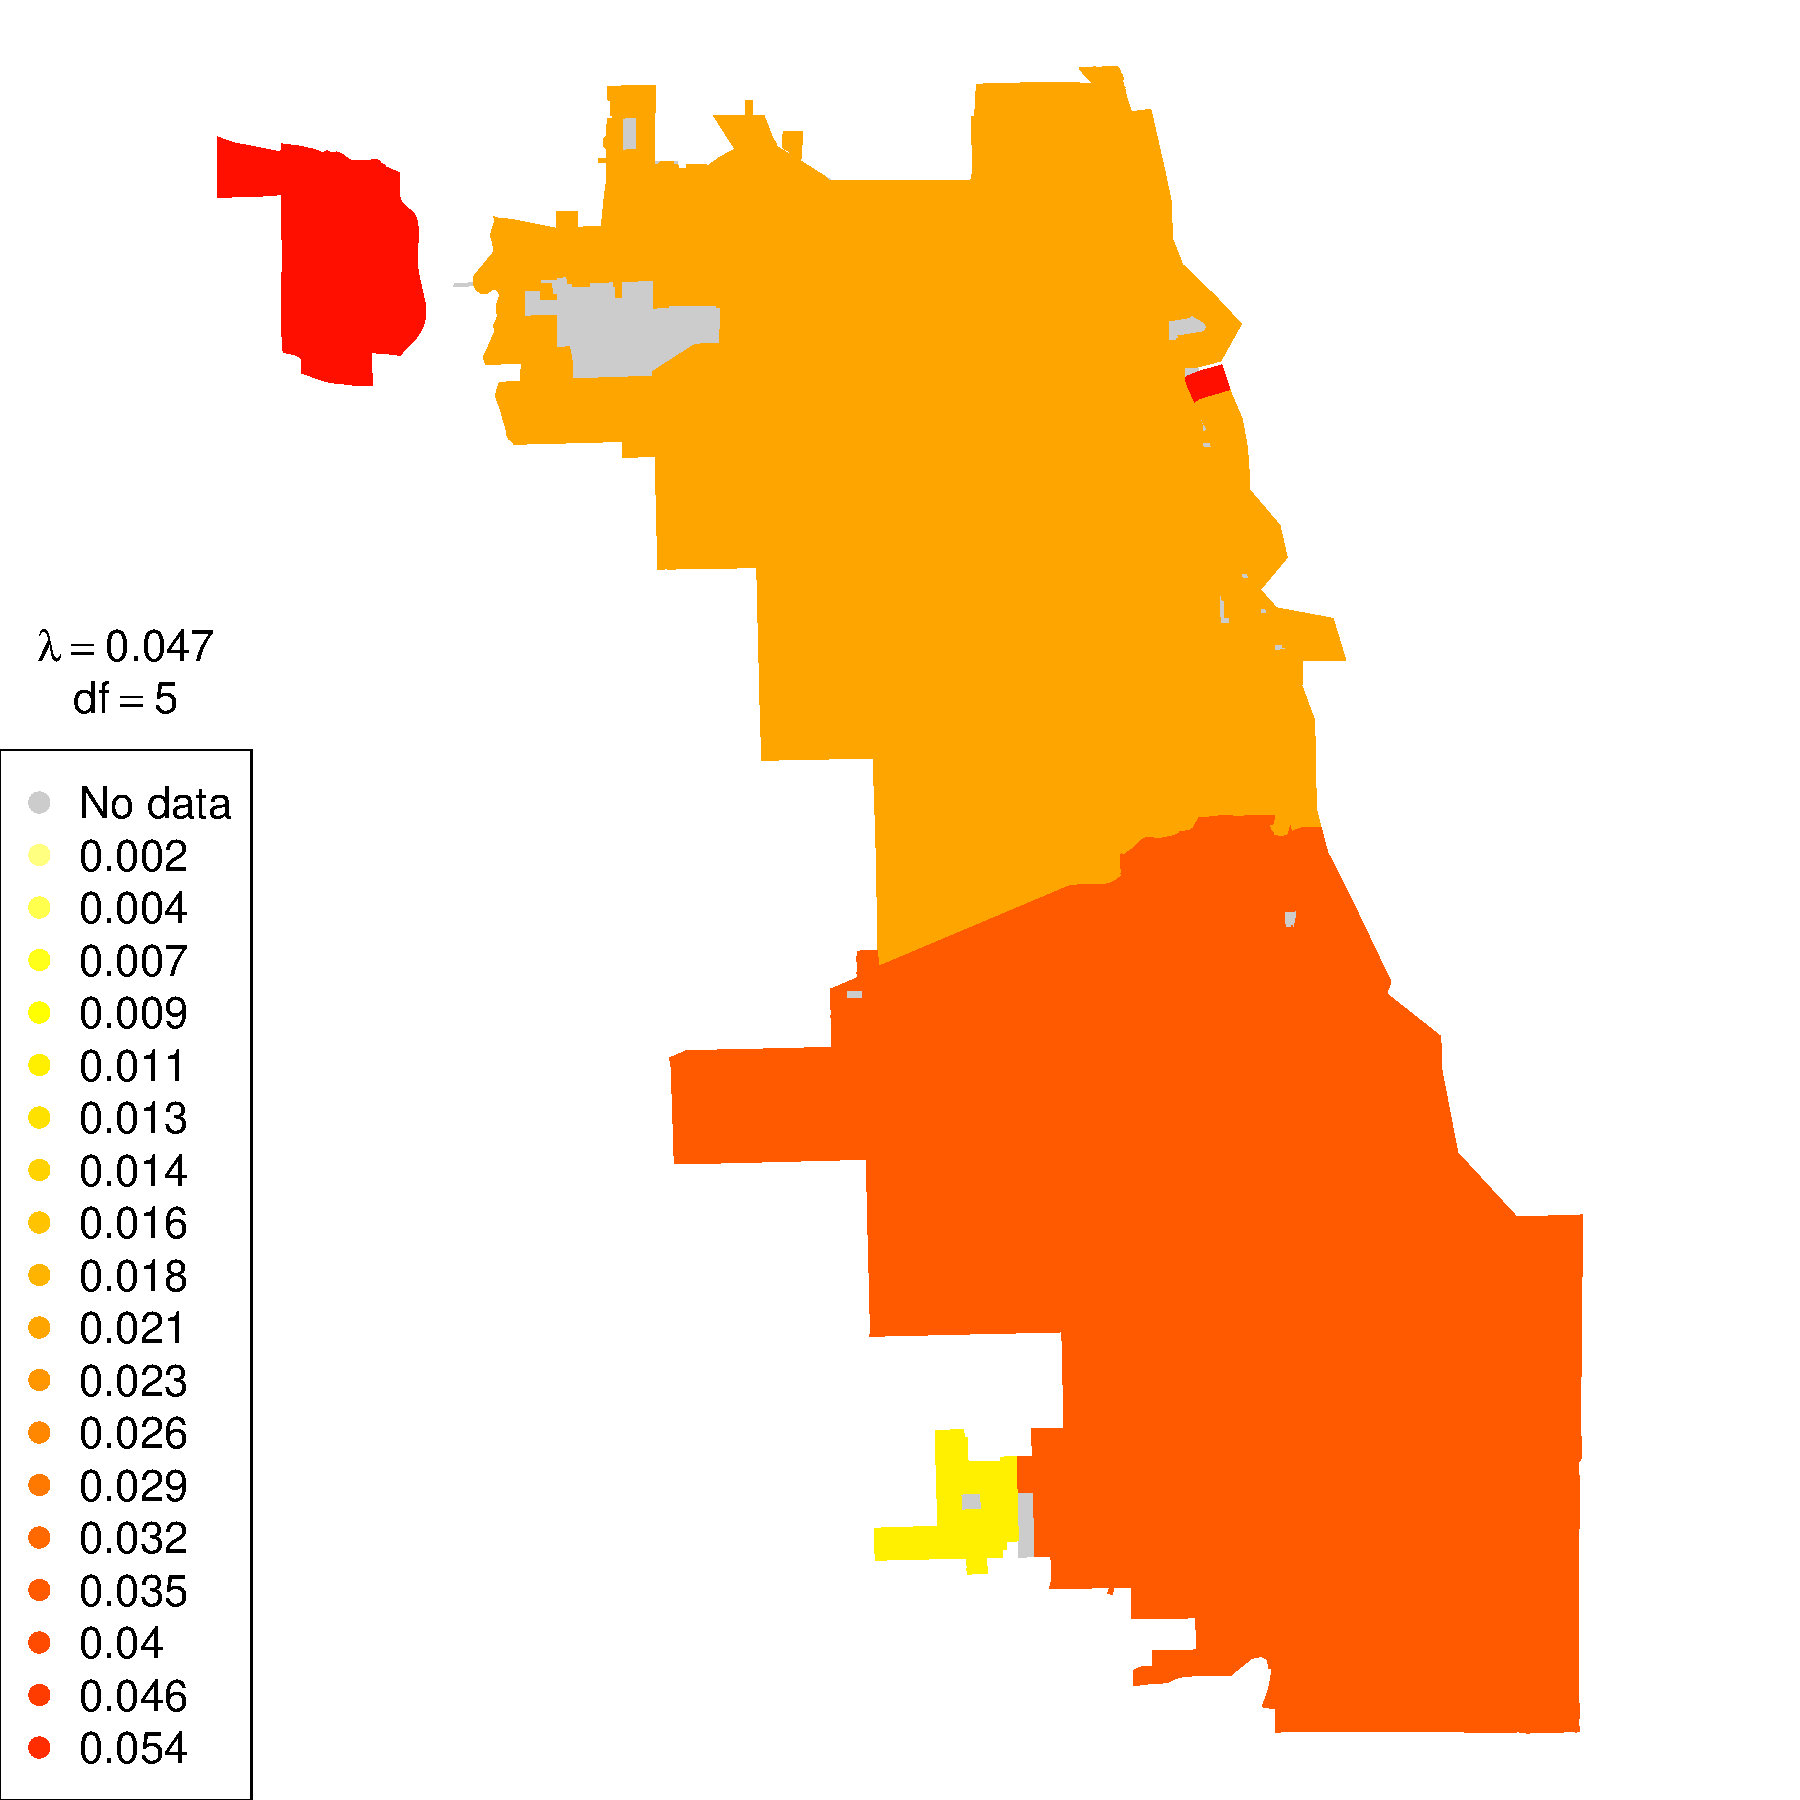
\includegraphics[height=\textheight]{img/chicago_rob_5df.pdf}

\end{frame}

%%%%%%%%%%%%%%%%%%%%%%%%%%%%%%%%%%%%%%%%%%%%%%%%%%%
\begin{frame}

  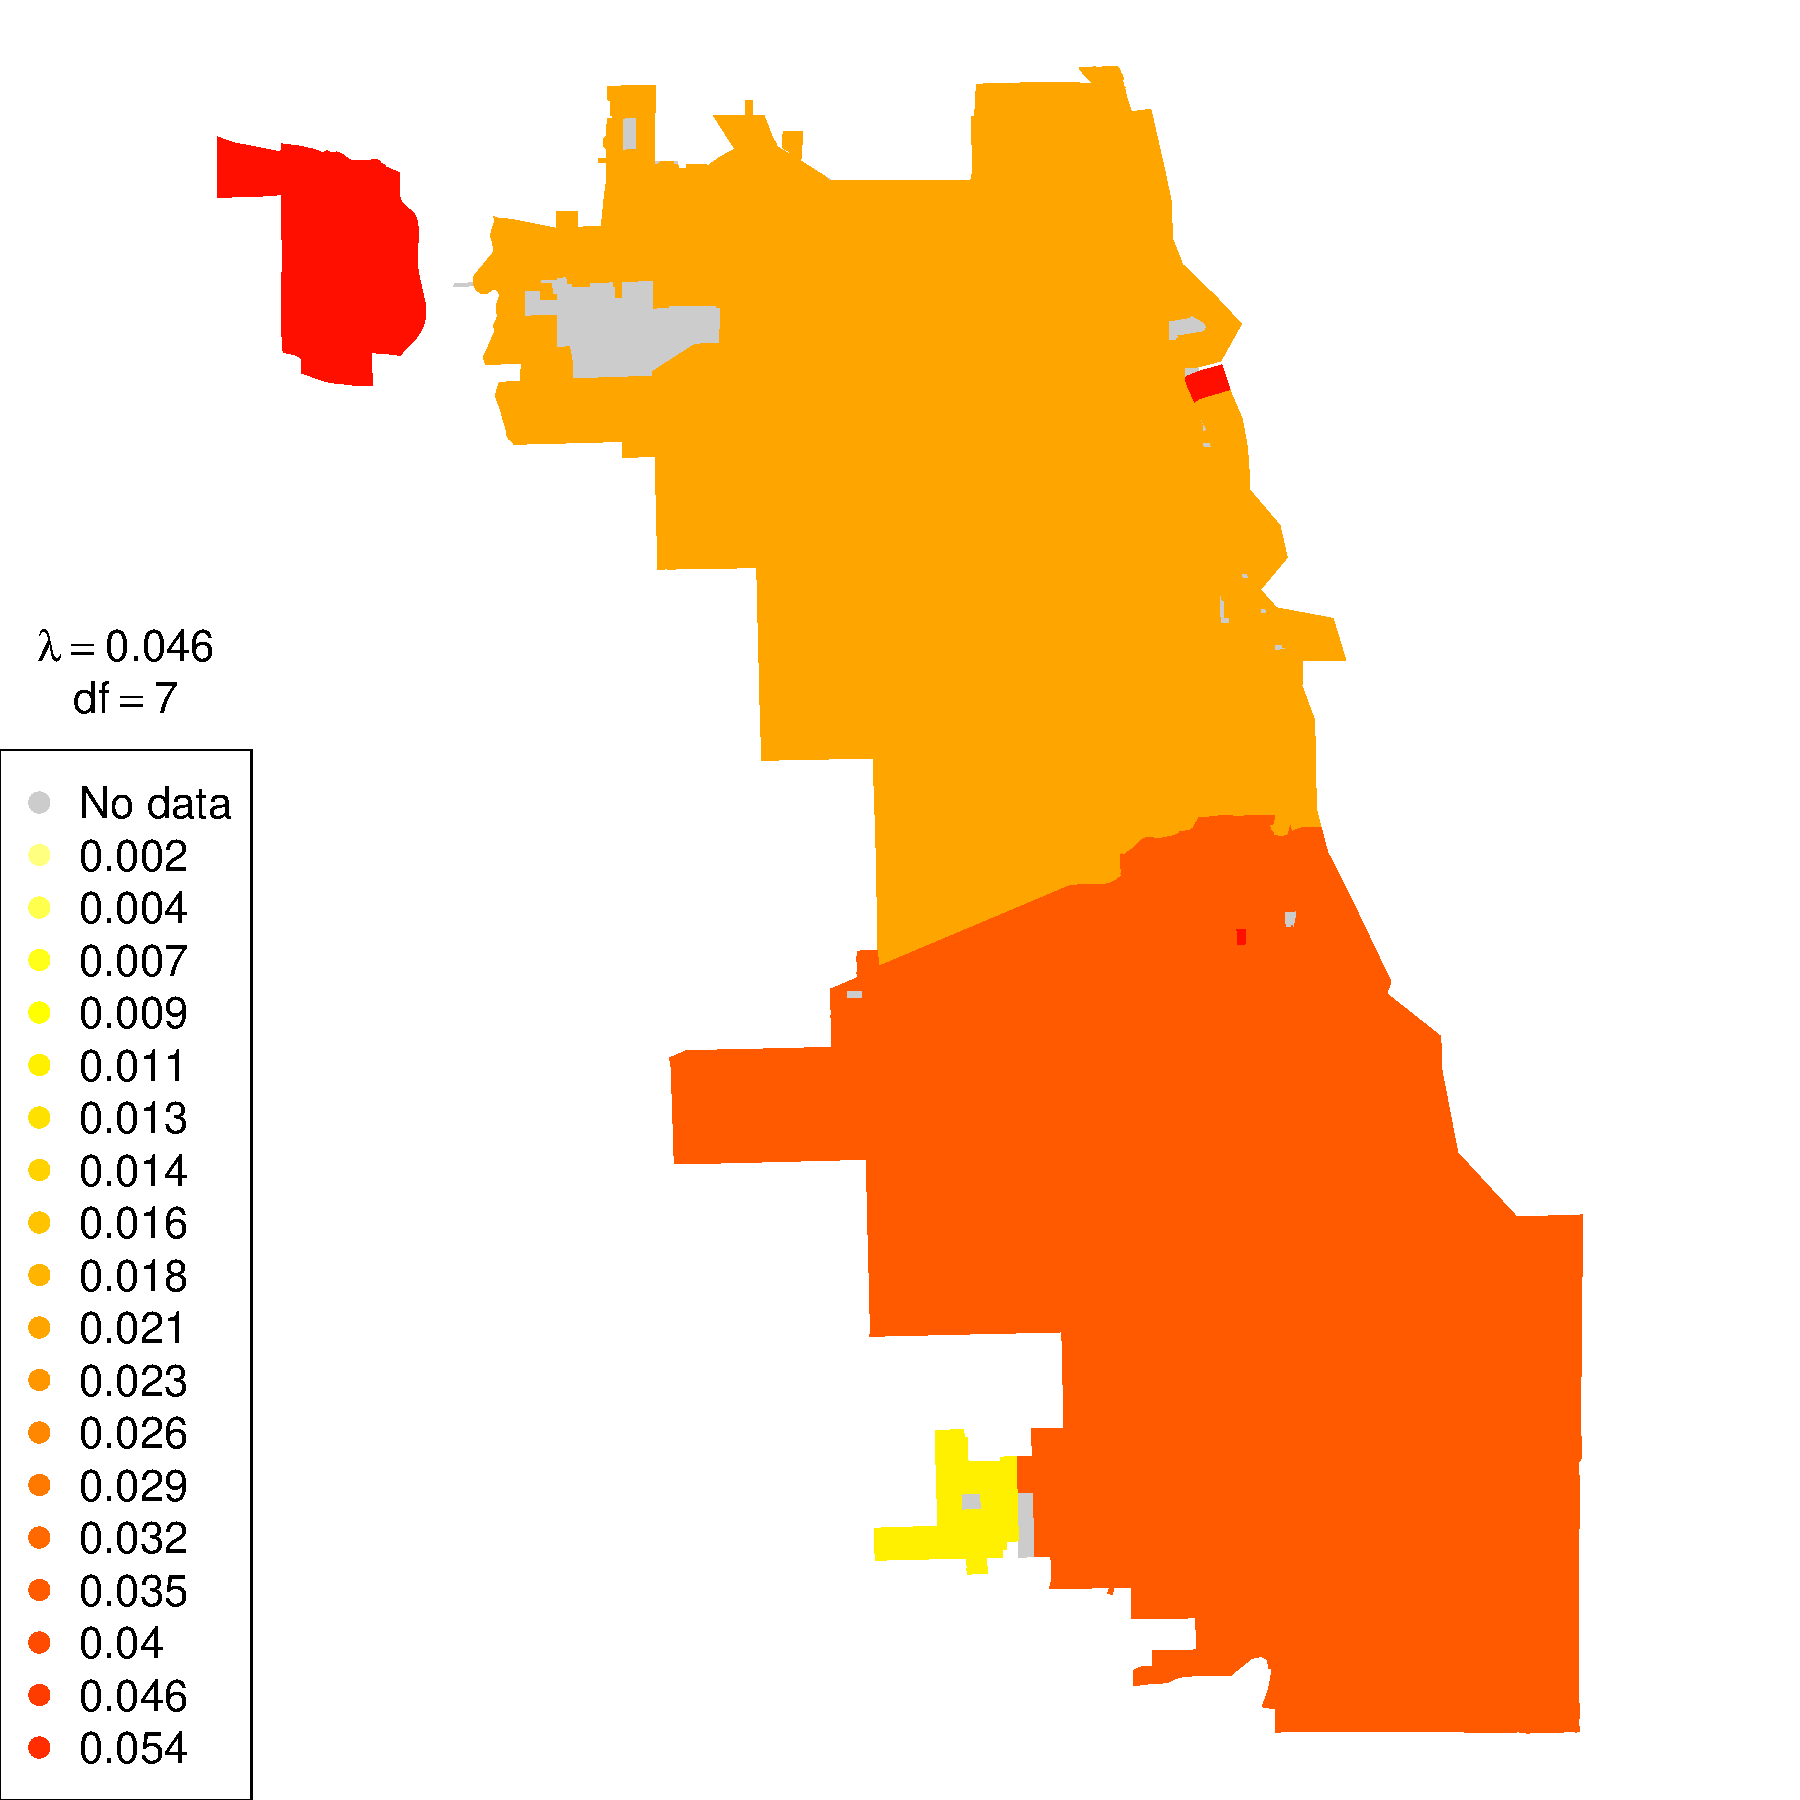
\includegraphics[height=\textheight]{img/chicago_rob_7df.pdf}

\end{frame}

%%%%%%%%%%%%%%%%%%%%%%%%%%%%%%%%%%%%%%%%%%%%%%%%%%%
\begin{frame}

  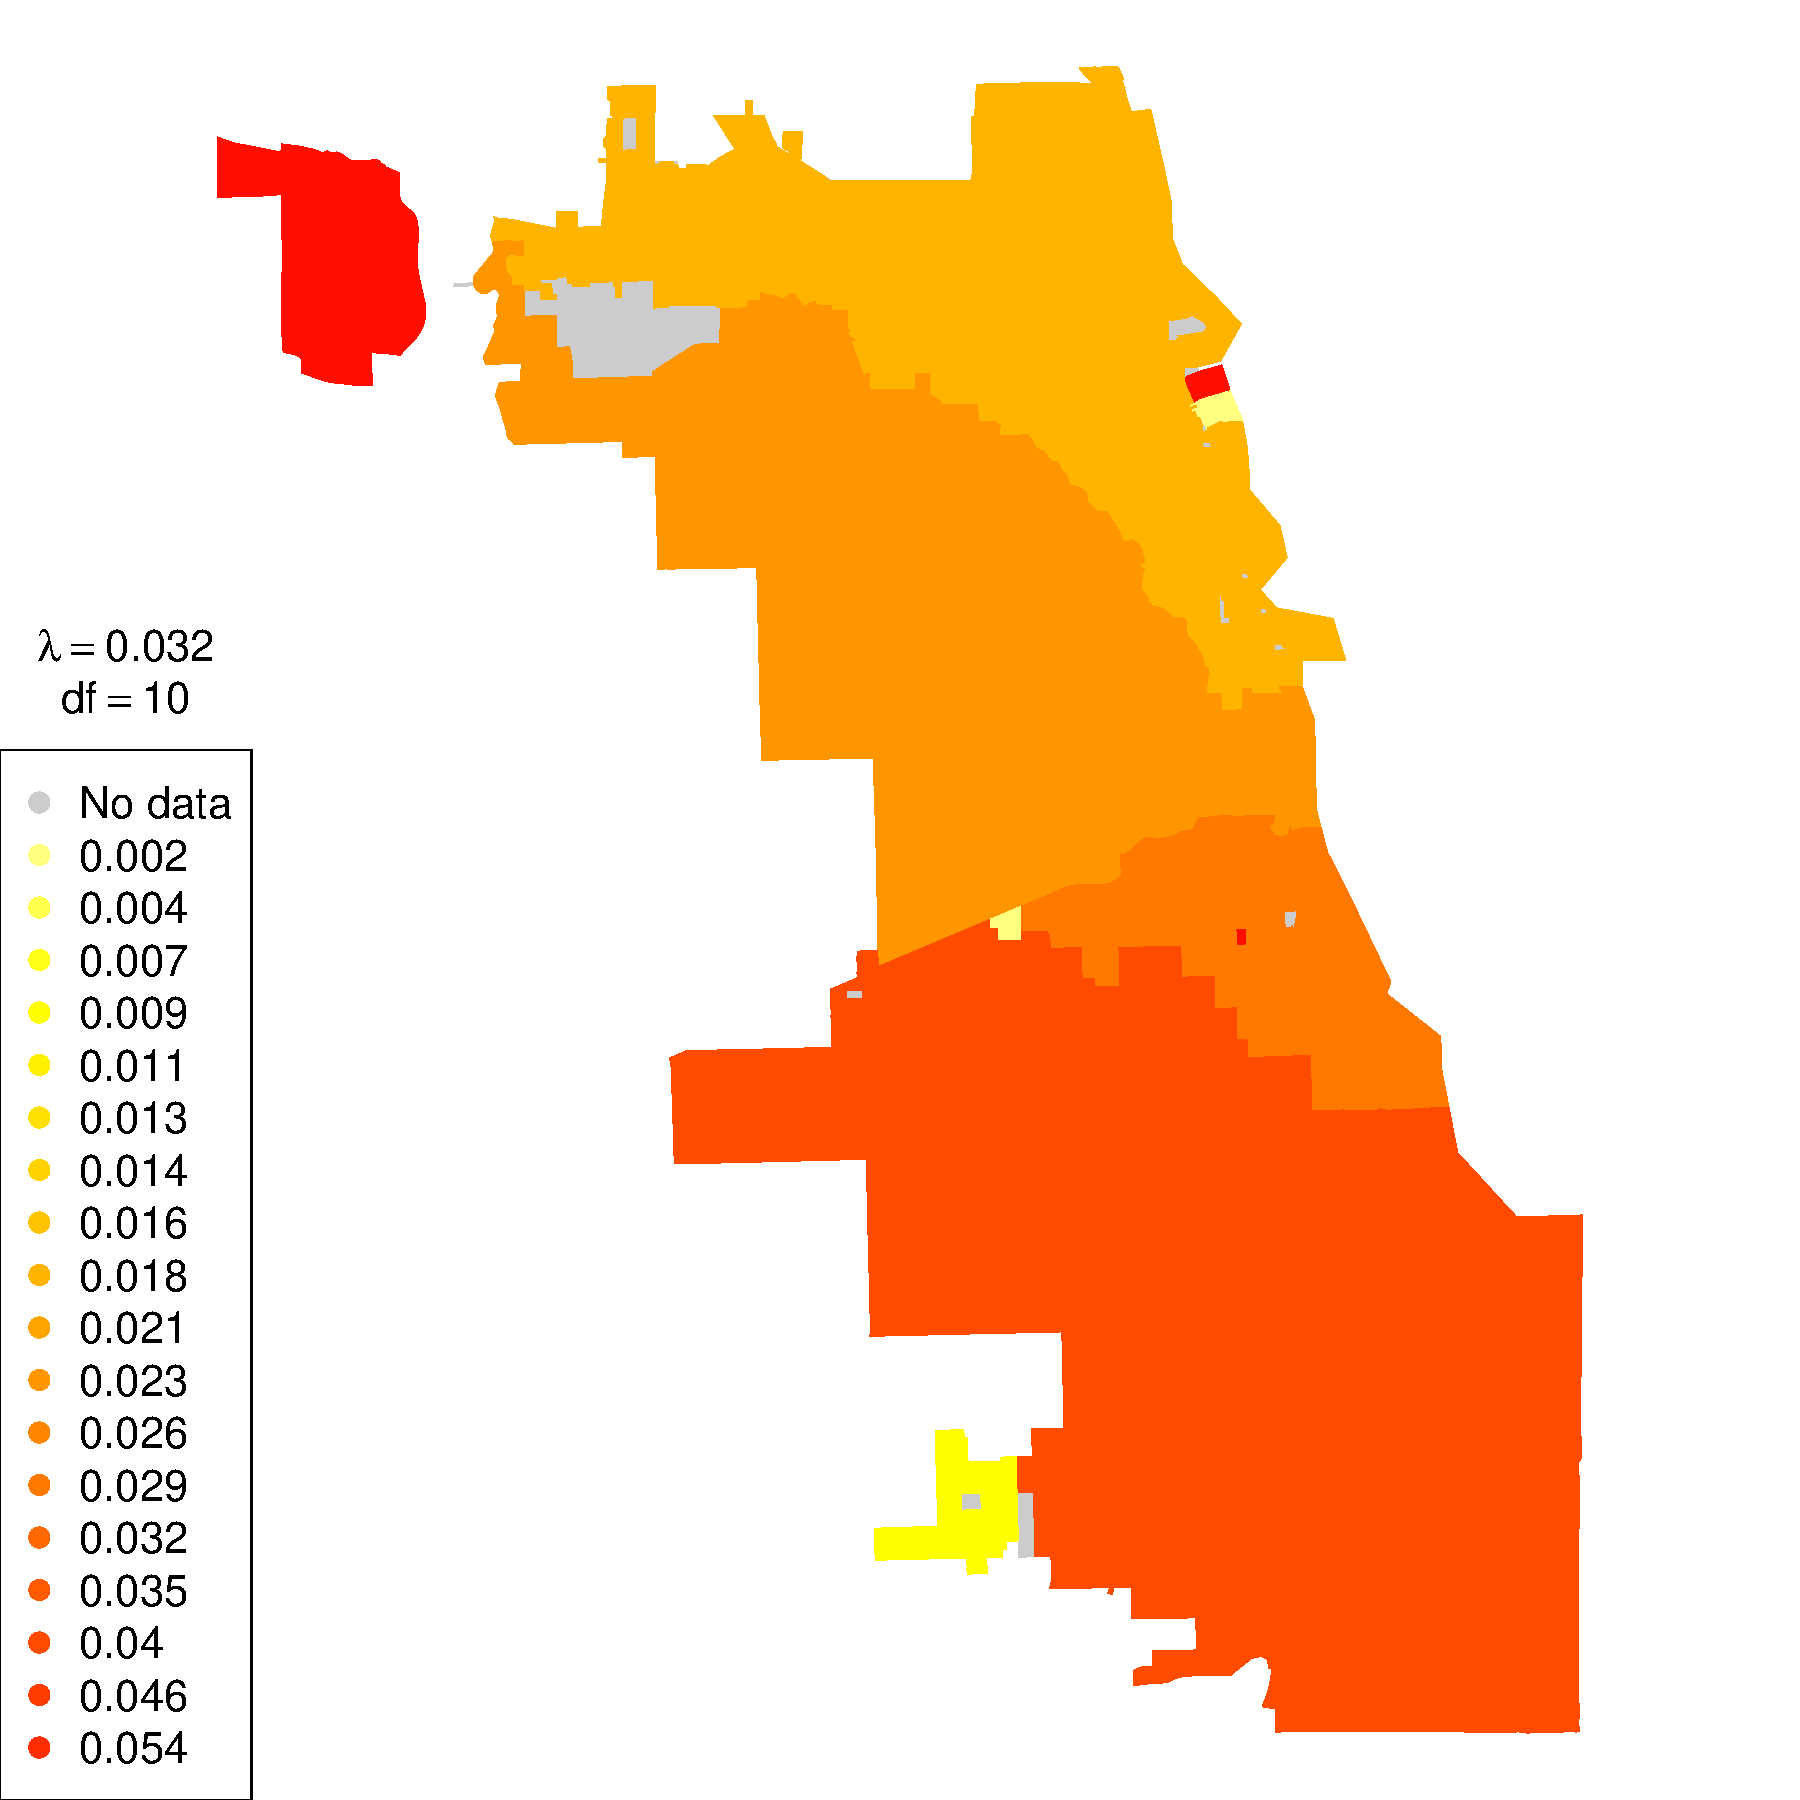
\includegraphics[height=\textheight]{img/chicago_rob_10df.pdf}

\end{frame}

%%%%%%%%%%%%%%%%%%%%%%%%%%%%%%%%%%%%%%%%%%%%%%%%%%%
\begin{frame}

  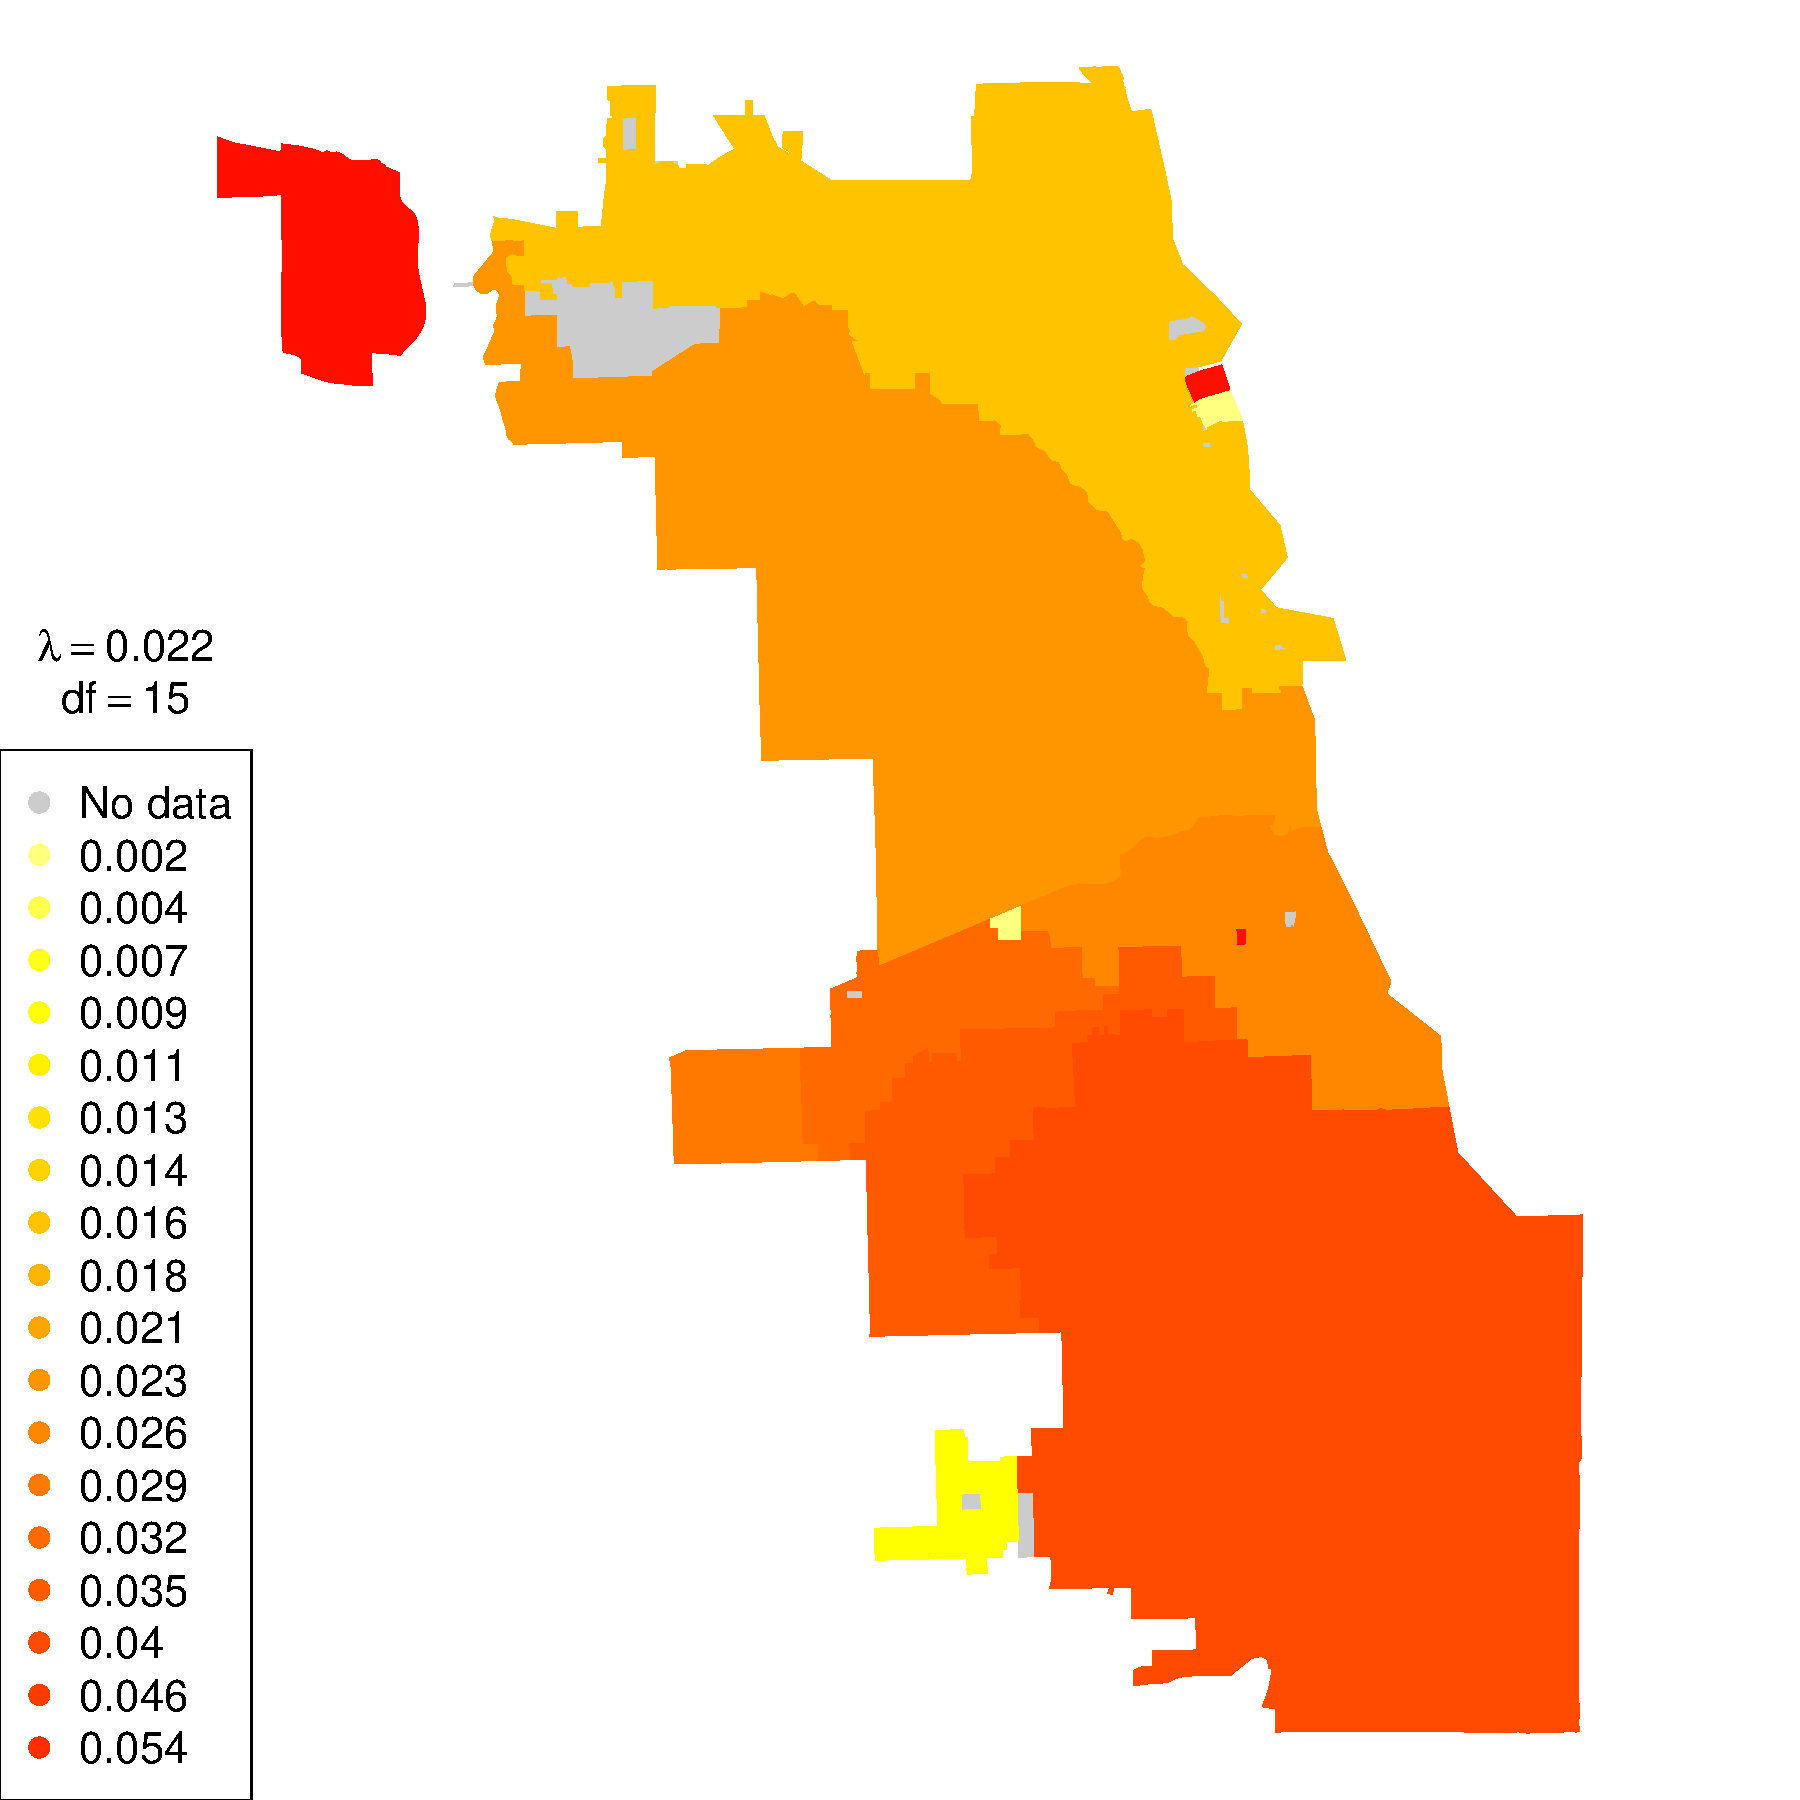
\includegraphics[height=\textheight]{img/chicago_rob_15df.pdf}

\end{frame}


%%%%%%%%%%%%%%%%%%%%%%%%%%%%%%%%%%%%%%%%%%%%%%%%%%%
\begin{frame}

  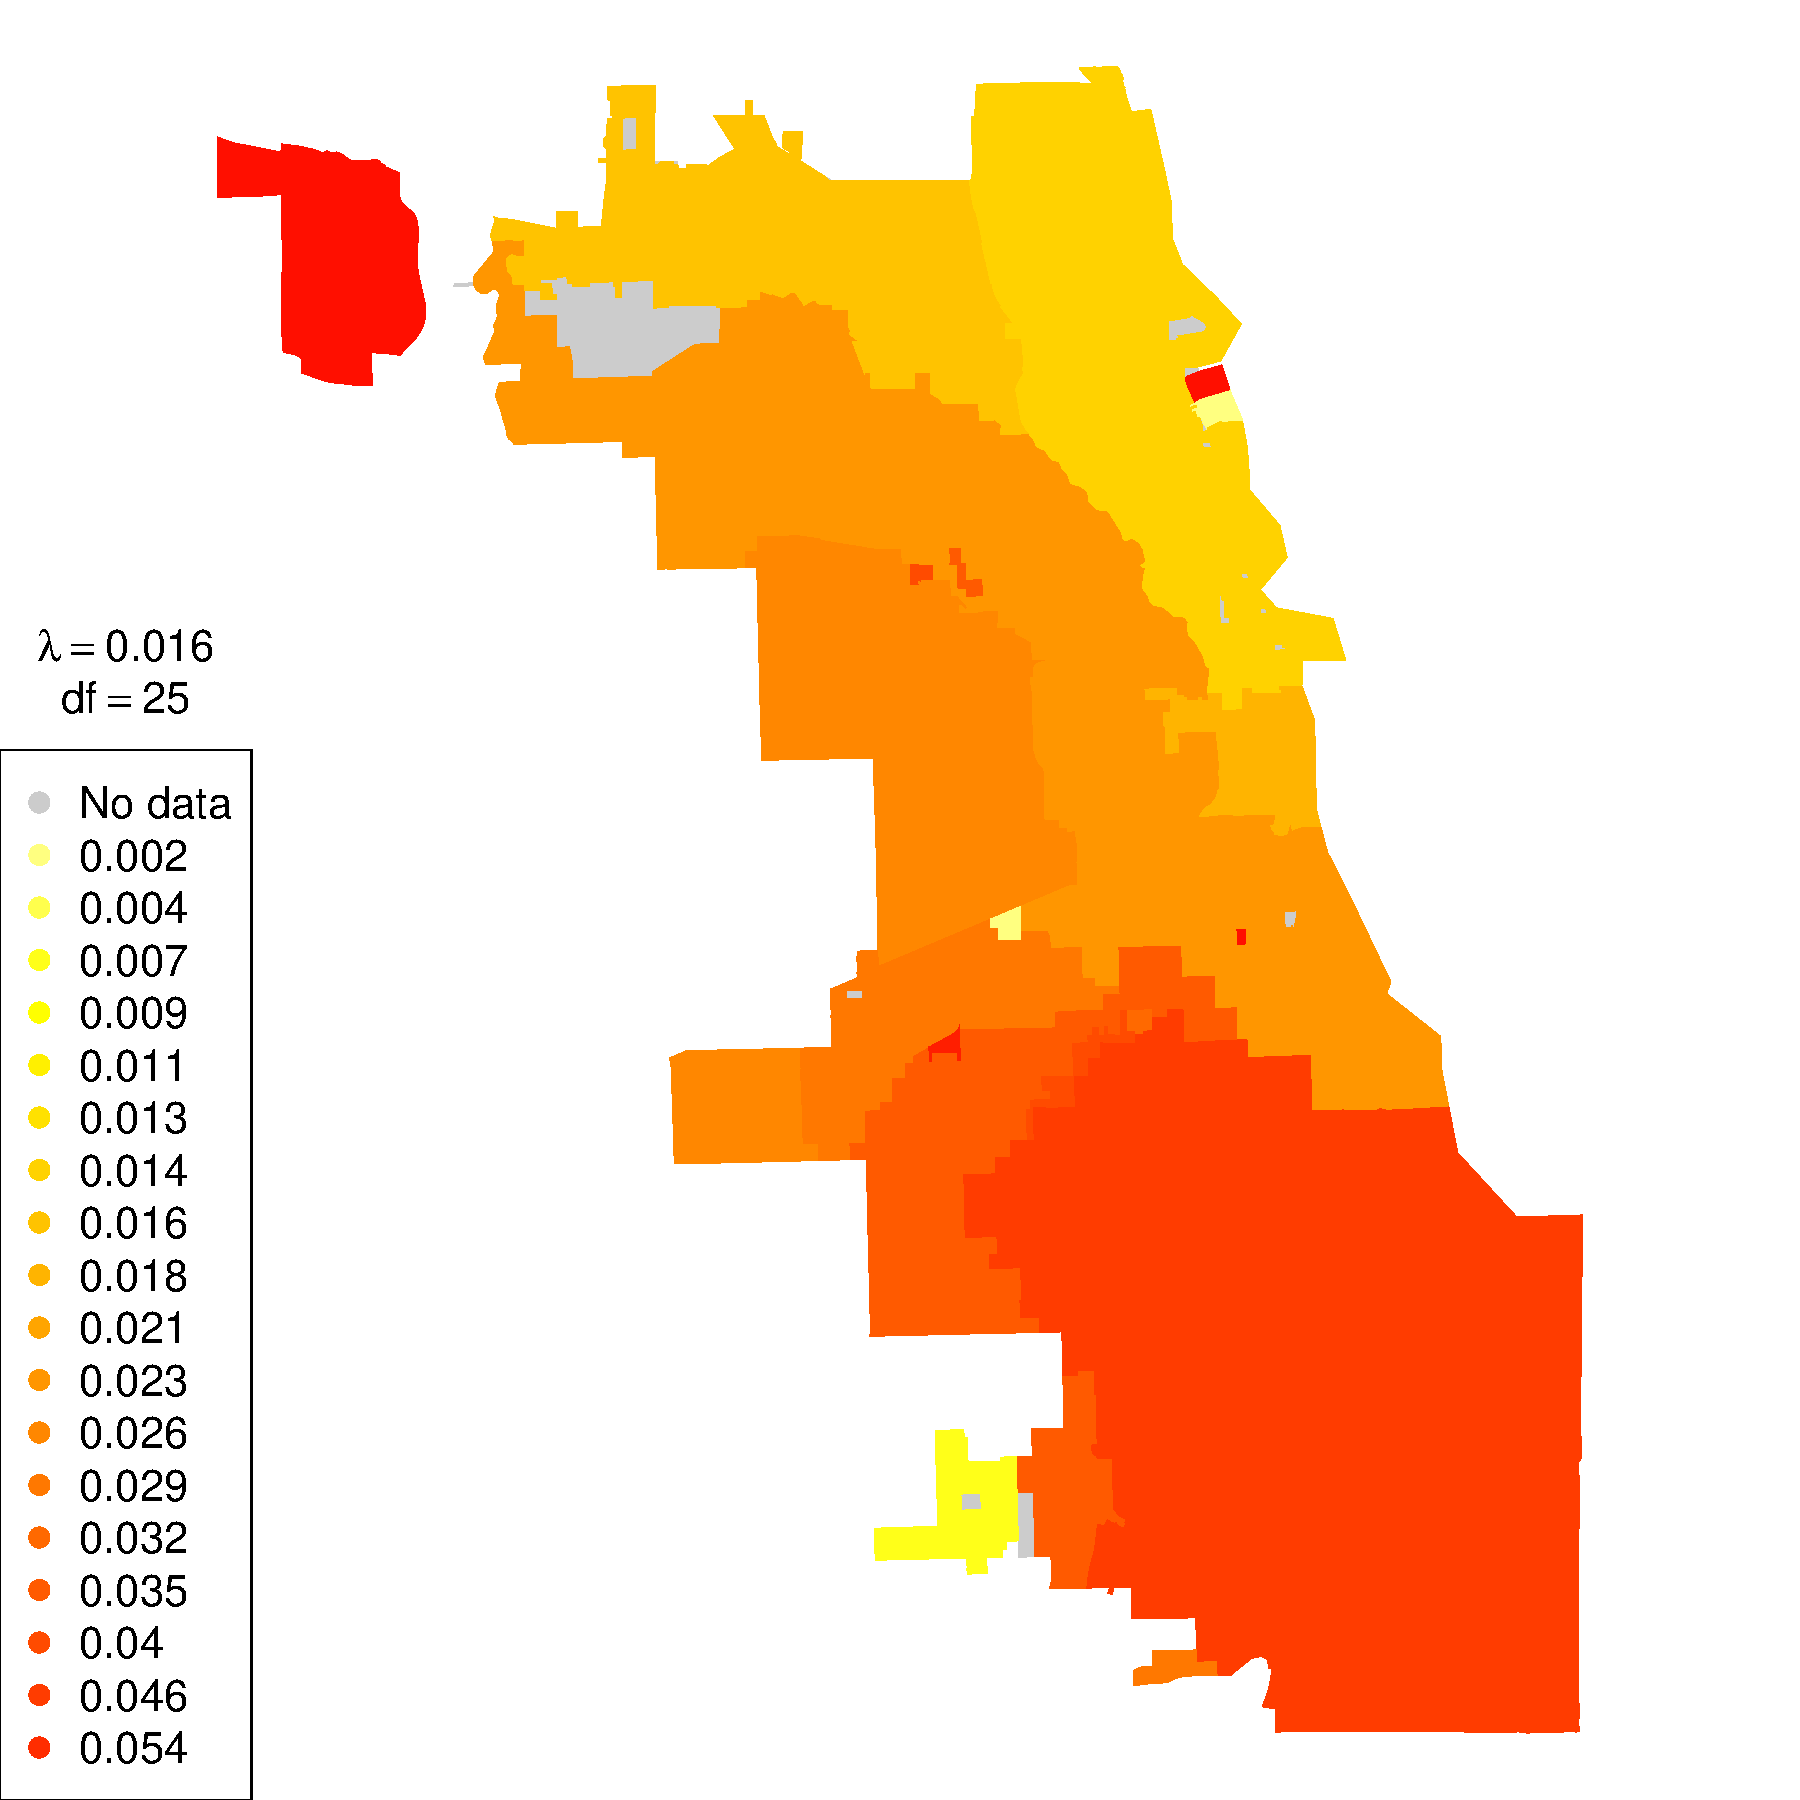
\includegraphics[height=\textheight]{img/chicago_rob_25df.pdf}

\end{frame}


%%%%%%%%%%%%%%%%%%%%%%%%%%%%%%%%%%%%%%%%%%%%%%%%%%%
\begin{frame}
  \frametitle{Sparse fused lasso}

A common variant of the fused lasso employs an additional $\ell_1$ penalty on
the coefficients themselves:
\begin{align*}
\widehat{\beta} &= \argmin_{\beta \in \mathbb{R}^n} \, \frac{1}{2} \sum_{i=1}^n (y_i-\beta_i)^2 +
\lambda \sum_{(i,j)\in E} |\beta_i-\beta_j| + \gamma \cdot \lambda \sum_{i=1}^n |\beta_i|.
\end{align*}
Here $\gamma \geq 0$ is another parameter that controls the ratio between the fusion
and sparsity penalty terms.

Note that this also fits into the generalized
lasso framework, as it simply concatenates (a multiple of) the identity matrix to the rows
of a fused lasso penalty matrix.

\end{frame}

%%%%%%%%%%%%%%%%%%%%%%%%%%%%%%%%%%%%%%%%%%%%%%%%%%%
\begin{frame}[fragile]

Take the following example:
\begin{verbatim}
> library(genlasso)
> set.seed(1)
> n = 100
> i = 1:n
> y = (i > 20 & i < 30) + 5*(i > 50 & i < 70) +
+   rnorm(n, sd=0.1)
> out = fusedlasso1d(y)
> beta1 = coef(out, lambda=1.5)$beta
\end{verbatim}
To calculate the soft thresholded solution, we apply soft thresholding to
the result:
\begin{verbatim}
beta2 = softthresh(out, lambda=1.5, gamma=1)
\end{verbatim}

\end{frame}

%%%%%%%%%%%%%%%%%%%%%%%%%%%%%%%%%%%%%%%%%%%%%%%%%%%
\begin{frame}

\begin{center}
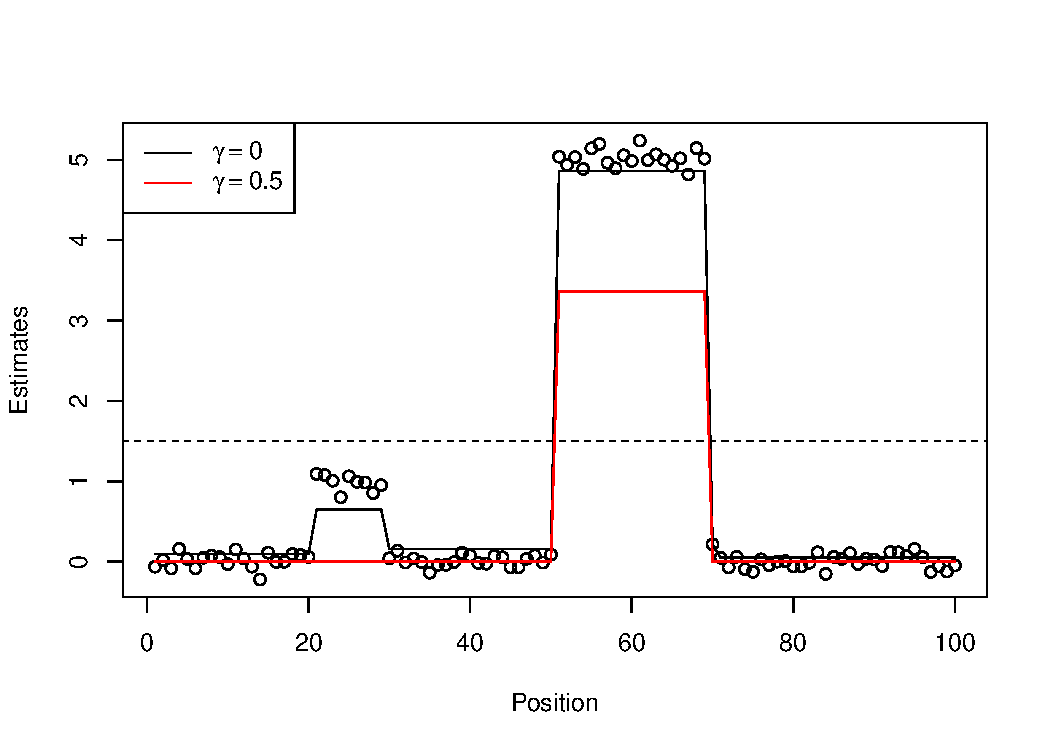
\includegraphics[width=\textwidth]{img/eq7x.pdf}
\end{center}

\end{frame}

%%%%%%%%%%%%%%%%%%%%%%%%%%%%%%%%%%%%%%%%%%%%%%%%%%%
\begin{frame}
  \frametitle{Trend filtering}
\small

Like the 1d fused lasso, trend filtering in the signal approximator case $X=I$ assumes
that the data $y=(y_1,\ldots y_n) \in \mathbb{R}^n$ is meaningfully ordered from $1$ to $n$,
and fits a piecewise polynomial of a specified degree. For example, linear trend filtering
(with $X=I$) solves the following minimization problem:
\begin{align}
\widehat{\beta} &= \argmin_{\beta \in \mathbb{R}^n} \, \frac{1}{2} \sum_{i=1}^n (y_i-\beta_i)^2 +
\lambda \sum_{i=1}^{n-2} |\beta_i - 2\beta_{i+1} + \beta_{i+1}|.
\end{align}
Notice that here the discrete second derivative is penalized, as opposed to the discrete
first derivative in the 1d fused lasso criterion. Quadratic and cubic
trend filtering are defined similarly, by penalizing the discrete third and fourth
derivative, respectively. (In this light, we can think of the 1d fused lasso as constant
or zeroth order trend filtering.)

\end{frame}


%%%%%%%%%%%%%%%%%%%%%%%%%%%%%%%%%%%%%%%%%%%%%%%%%%%
\begin{frame}
  \frametitle{References}
  \footnotesize

  \begin{itemize}
  \item Robert Tibshirani, et al. {\it Sparsity and smoothness via the fused lasso.}
  Journal of the Royal Statistical Society: Series B (Statistical Methodology), 67: 91–108.
  \item Ryan Tibshirani and
  Taylor Arnold (2014). {\it genlasso: Path algorithm for generalized lasso problems.}
  R package version 1.2.
  \item  S. Boyd et al.,
  {\it Distributed optimization and statistical learning via the alternating
  direction method of multipliers}. Foundations and Trends in Machine Learning,
  3(1):1–122, 2011.
  \item Ryan Tibshirani and J. Taylor (2011). "The solution path of the
     generalized lasso", Annals of Statistics 39 (3) 1335-1371.
  \end{itemize}
\end{frame}



\end{document}











